%%%%%%%%%%%%%%%%%%%%%%%%%%%%%%%%%%%%%%%%%%%%%%%%%%%%%%%%%%%%%%%%%%%%%%%%%%%%%%%
% Memorial para concurso público de Pesquisador Adjunto I em Sismologia.
%
% Formatação inspirada em:
% * https://github.com/leouieda/memorial2023
% * https://github.com/birocoles/memos

%%%%%%%%%%%%%%%%%%%%%%%%%%%%%%%%%%%%%%%%%%%%%%%%%%%%%%%%%%%%%%%%%%%%%%%%%%%%%%%

%%%%%%%%%%%%%%%%%%%%%%%%%%%%%%%%%%%%%%%%%%%%%%%%%%%%%%%%%%%%%%%%%%%%%%%%%%%%%%%
% Set a class and import packages
\documentclass[10pt,a4paper,oneside]{book}

% Variables
\newcommand{\Year}{2024}
\newcommand{\Author}{Diogo Luiz de Oliveira Coelho}
\newcommand{\Title}{Memorial de \Author{} para concurso público - Pesquisador Adjunto I em Sismologia - ON/MCTI}
\newcommand{\Email}{diogoloc@on.br}
\newcommand{\EmailPersonal}{locdiogo@gmail.com}
\newcommand{\ORCID}{0000-0001-5426-0455}
\newcommand{\ResearchGate}{https://www.researchgate.net/profile/Diogo-De-Oliveira-Coelho}
\newcommand{\Lattes}{4330106475199471}

% Import packages
\usepackage[utf8]{inputenc}
\usepackage[T1]{fontenc}
\usepackage[brazil]{babel}
\usepackage{geometry}
\usepackage{graphicx}
\usepackage{amssymb}
\usepackage{amsmath}
\usepackage{mathpazo}
\usepackage{hyperref}
% create fancy headers
\usepackage{fancyhdr}
% commands for managing dates and its formats
\usepackage{datetime2}
% improved urls with proper hyphenation
\usepackage{xurl}
% Control over enumerate and itemize
\usepackage{enumitem}
% Tweak the look of captions
\usepackage{caption}
% To control the style of section titles
\usepackage{titlesec}
% Add the bibliography to the table of contents
\usepackage[nottoc,chapter]{tocbibind}
\usepackage[round,authoryear,sort]{natbib}
% show dois as links on references
\usepackage{doi}
% Icon and fonts (requires using xelatex or luatex)
\usepackage{fontawesome5}
\usepackage{academicons}
\usepackage{fontspec}
\usepackage[mono]{notomath}
% To make everything neater
\usepackage{microtype}
% To make fancy text boxes
\usepackage{xcolor}
\usepackage[framemethod=default]{mdframed}
% For fancy and multipage tables
\usepackage{tabularx}
\usepackage{ltablex}
% To define custom environments
\usepackage{environ}
\usepackage{setspace}
% Reference sections by name
\usepackage{nameref}
% Better handling of footnotes inside summary boxes
\usepackage{footmisc}

%to rotate the page
\usepackage{pdflscape}

%To plot piechart
\usepackage{bera}
\usepackage{pstricks-add}
\usepackage{pgf-pie}

%%%%%%%%%%%%%%%%%%%%%%%%%%%%%%%%%%%%%%%%%%%%%%%%%%%%%%%%%%%%%%%%%%%%%%%%%%%%%%%

%%%%%%%%%%%%%%%%%%%%%%%%%%%%%%%%%%%%%%%%%%%%%%%%%%%%%%%%%%%%%%%%%%%%%%%%%%%%%%%
% Configuration of the document

\geometry{%
  left=30mm,
  right=30mm,
  top=20mm,
  bottom=15mm,
  headsep=5mm,
  headheight=5mm,
  footskip=10mm,
  includehead=true,
  includefoot=true
}

% Increase the line spacing
\SetSinglespace{1.2}
\onehalfspacing

% Remove spacing between enumerate/itemize items
\setlist{nosep}

% Padding between the first figure and the chapter title
\newcommand{\HeroFigPad}{\vspace{-1cm}}

% Padding before the software logo figures
\newcommand{\SoftwareFigPad}{\vspace{-0.3cm}}

% Add a link to a DOI
\newcommand{\DOI}[1]{\url{https://doi.org/#1}}

% Add a link to a GitHub repository
\newcommand{\GitHub}[1]{\faGithub{} Código: \url{https://github.com/#1}}

% Add a link to a YouTube video
\newcommand{\YouTube}[1]{\faYoutube{} Vídeo: \url{https://youtu.be/#1}}

% Add a link to a supplementary data
\newcommand{\Data}[1]{\faChartBar{} Dados: \url{https://doi.org/#1}}

% Add a link to a preprint
\newcommand{\Preprint}[1]{\faLockOpen{} Preprint: \url{https://doi.org/#1}}

% Make a Unicode bullet symbol
\newcommand{\Bullet}{•\enspace}

% Define custom colors
\definecolor{lu_gray}{gray}{0.98}
\definecolor{lu_darkgray}{gray}{0.3}
\definecolor{gold(metallic)}{rgb}{0.83, 0.69, 0.22}
\definecolor{cornsilk}{rgb}{1.0, 0.97, 0.86}
\definecolor{lu_blue}{RGB}{32, 96, 194}
\definecolor{lu_lightblue}{RGB}{238, 245, 250}
\definecolor{timberwolf}{rgb}{0.86, 0.84, 0.82}
\definecolor{battleshipgrey}{rgb}{0.52, 0.52, 0.51}

% Customize how Chapter headings are displayed
\titleformat{\chapter}[display]{\normalfont}{\large Capítulo \thechapter}{0pt}{\huge}[\titlerule]
\titlespacing*{\chapter}{0pt}{-40pt}{40pt}

% Set the spacing between bibliography entries (requires natbib)
\setlength{\bibsep}{0pt}

% Configure captions
\captionsetup{labelfont=bf,font={small,color=lu_darkgray},skip=0pt}

% Define a fancy text box
\mdfdefinestyle{summarybox}{%
  leftline=true,
  rightline=false,
  topline=false,
  bottomline=false,
  linewidth=4pt,
  linecolor=gold(metallic),
  frametitlefont=\bfseries\color{black}\small,
  frametitlebackgroundcolor=cornsilk,
  frametitleaboveskip=7pt,
  frametitlebelowskip=7pt,
  frametitlerule=true,
  frametitlerulewidth=1pt,
  backgroundcolor=lu_gray,
  innertopmargin=7pt,
  innerbottommargin=10pt,
  innerleftmargin=15pt,
  innerrightmargin=15pt,
  skipbelow=5pt,
  skipabove=0pt,
}
\newmdenv[style=summarybox]{summarybox}
\mdfdefinestyle{subsummarybox}{%
  leftline=true,
  rightline=false,
  topline=false,
  bottomline=false,
  linewidth=4pt,
  linecolor=battleshipgrey,
  frametitlefont=\bfseries\color{black}\small,
  frametitlebackgroundcolor=timberwolf,
  frametitleaboveskip=7pt,
  frametitlebelowskip=7pt,
  frametitlerule=true,
  frametitlerulewidth=1pt,
  backgroundcolor=lu_gray,
  innertopmargin=7pt,
  innerbottommargin=10pt,
  innerleftmargin=15pt,
  innerrightmargin=15pt,
  skipbelow=5pt,
  skipabove=0pt,
}
\newmdenv[style=subsummarybox]{subsummarybox}

% Define something like an fa-ul and a date list
\NewEnviron{fa-ul}{%
  \vspace{-0.4cm}
  \small
  \renewcommand{\arraystretch}{1.25}
  \begin{tabularx}{\linewidth}{@{}p{0.05\linewidth}@{}@{}p{0.95\linewidth}@{}}
    \BODY
  \end{tabularx}%
}
\NewEnviron{datelist}{%
  \vspace{-0.4cm}
  \small
  \renewcommand{\arraystretch}{1.25}
  \begin{tabularx}{\linewidth}{@{}p{0.15\linewidth}@{}@{}p{0.85\linewidth}@{}}
    \BODY
  \end{tabularx}%
}
\NewEnviron{paperlist}{%
  \vspace{-0.4cm}
  \small
  \renewcommand{\arraystretch}{1.25}
  \begin{tabularx}{\linewidth}{@{}p{0.08\linewidth}@{}@{}p{0.92\linewidth}@{}}
    \BODY
  \end{tabularx}%
}
\NewEnviron{courselist}{%
  \vspace{-0.4cm}
  \small
  \renewcommand{\arraystretch}{1.25}
  \begin{tabularx}{\linewidth}{@{}p{0.15\linewidth}@{}@{}p{0.85\linewidth}@{}}
    \BODY
  \end{tabularx}
}

% Define a fancy enumerate that has a title
\NewEnviron{fancyenum}[2]{%
  \vspace{0.25cm}
  \noindent#1\quad\textbf{#2}:
  \vspace{0.25cm}
  \begin{enumerate}
    \BODY
  \end{enumerate}
}

% Configure hyperref and add PDF metadata
\hypersetup{
    colorlinks,
    allcolors=lu_blue,
    pdftitle={\Title},
    pdfauthor={\Author},
    pdftex,
    breaklinks=true,
}

% make urls use the same font as every other text
\urlstyle{same}

% Prevent footnotes from being broken into multiple pages
\interfootnotelinepenalty=10000

% Configure headers and footers
\fancyhf{}
\lhead{\fontsize{9pt}{0}\selectfont\itshape \nouppercase\leftmark}
\chead{}
\rhead{\fontsize{9pt}{0}\selectfont \thepage}
\cfoot{}
\renewcommand{\headrulewidth}{0.3pt}
%%%%%%%%%%%%%%%%%%%%%%%%%%%%%%%%%%%%%%%%%%%%%%%%%%%%%%%%%%%%%%%%%%%%%%%%%%%%%%%

%%%%%%%%%%%%%%%%%%%%%%%%%%%%%%%%%%%%%%%%%%%%%%%%%%%%%%%%%%%%%%%%%%%%%%%%%%%%%%%
\begin{document}

\pagestyle{plain}
\frontmatter

\begin{titlepage}
  \begin{center}
    \includegraphics[height=0.5cm]{images/logo_seismo.png}
    \vspace{1cm}

    CONCURSO PÚBLICO
    
    PESQUISADOR ADJUNTO I EM SISMOLOGIA
    
    OBSERVATÓRIO NACIONAL

    \vspace{5cm}

    \textbf{\LARGE Memorial}
    \vspace{1cm}

    \textbf{\LARGE \MakeUppercase{\Author{}}}
    \vspace{5cm}

    {\small
	Apresentado para concurso público de provas e títulos para cargo de

	Pesquisador Adjunto I em Sismologia à Coordenação de Geofísica do

	Observatório Nacional.
      \vspace{1cm}

	EDITAL N$^{\circ}$   1, DE 9 DE OUTUBRO DE 2023
    }
    \vfill

    \Year{}
  \end{center}
\end{titlepage}

%==============================================================================
\chapter*{Resumo}

Ao longo da minha trajetória acadêmica, conclui o bacharelado em \href{https://geologia.ufes.br/}{Geologia} pela Universidade Federal do Espírito Santo, o mestrado em \href{https://www.gov.br/observatorio/pt-br/assuntos/programas-academicos/pos-graduacao-em-geofisica/pos-graduacao-em-geofisica}{Geofísica} pelo Observatório Nacional e o doutorado em \href{https://posgraduacao.ufrn.br/325}{Geodinâmica e Geofísica} pela Universidade Federal do Rio Grande do Norte. Durante minha formação acadêmica, tive a oportunidade de passar por três instituições de ensino superior ligadas ao Ministério da Educação (MEC), uma unidade de pesquisa vinculada ao Ministério da Ciência, Tecnologia e Inovação (MCTI), além de realizar estágio de nível superior na Petrobras, uma empresa estatal do setor de energia. Nessa caminhada acadêmica, tive a oportunidade enriquecedora de vivenciar de perto o funcionamento de instituições públicas em quatro estados distintos do país. Essa diversidade geográfica proporcionou-me um aprendizado valioso e o aprimoramento da minha atuação na academia. Desde minha entrada no Observatório Nacional, ministrei a disciplina de \href{https://www.gov.br/observatorio/pt-br/assuntos/programas-academicos/pos-graduacao-em-geofisica/grade-curricular}{Introdução à Sismologia} em nível de pós-graduação, cursos de curta duração para graduandos em outras instituições e orientei alunos de iniciação científica. No âmbito da divulgação e popularização da ciência, participei de mais de 35 eventos relacionados a popularização e divulgação da ciência, dentre feiras de tecnologia, entrevistas para diversos canais da imprensa, \textit{podcast}, revisão de textos e notas técnicas explorando temas variados da sismologia, incluindo sua relação com desastres naturais, bem como curiosidades gerais da população sobre a atuação de um pesquisador em geofísica. Desde o mestrado, tenho atuado na área da sismologia e da tectônica da Crosta. Já no doutorado iniciei, de forma sistemática, o desenvolvimento de diversos códigos computacionais, estes relacionados à estruturação do manto terrestre e ao processamento de dados oriundos de redes subaquáticas. Este memorial apresenta de forma resumida minha formação e atuação acadêmica, incluindo algumas considerações sobre os fatores que influenciaram na minha trajetória e os principais ensinamentos adquiridos ao longo dessa jornada que me ajudaram a fazer pequenos ajustes na rota até aqui.

\begin{landscape}
% Conteúdo da página em modo paisagem
\begin{figure}[tb]
  \begin{center}
    \includegraphics[width=\pagewidth]{images/linha_do_tempo.png}
  \end{center}
  \caption*{
    Resumo da minha trajetória acadêmica, desde a entrada na graduação em Geologia na Universidade Federal do Espírito Santo em 2007 até meu terceiro estágio pós-doutoral no Observatório Nacional no ano de 2024.
    }
\end{figure}
\end{landscape}
%==============================================================================
\tableofcontents

\mainmatter
\pagestyle{fancy}

%==============================================================================
\chapter{Apresentação}

\begin{figure}[h]
  \HeroFigPad
  \begin{center}
    \includegraphics[width=\textwidth]{images/vasco.jpeg}
  \end{center}
  \caption{
    Visitando em 2023 o estádio de \href{https://vasco.com.br/sao-januario/}{São Januário}, a colina histórica. Por estar localizada a menos de 1 km do Observatório Nacional, a sede do Vasco da Gama foi um dos principais fatores que me motivaram a entrar no programa de pós-graduação do Observatório Nacional em 2013.
  }
  \label{fig_riacho}
\end{figure}

Este memorial apresenta uma análise sumária sobre a minha trajetória acadêmica, contemplando formação, atuação, atividades de ensino e divulgação/popularização da ciência.
\bigskip

\begin{summarybox}[frametitle=\faIcon{address-card}{}\quad Informações para contato]
  \begin{fa-ul}
    \faIcon{at} & email profissional: \href{mailto:\Email}{\Email} \\
    \faIcon{at} & email pessoal: \href{mailto:\EmailPersonal}{\EmailPersonal} \\
    \aiOrcid & ORCID: \href{https://orcid.org/\ORCID}{\ORCID} \\
    \aiResearchGate & ResearchGate: \href{\ResearchGate}{\ResearchGate} \\
    \aiLattes & Currículo Lattes: \url{https://lattes.cnpq.br/\Lattes} \\
    \faIcon{github} & Github: \url{https://github.com/diogoloc}
  \end{fa-ul}
\end{summarybox}

Passei a maior parte da minha infância e juventude no extremo norte fluminense, mais precisamente em \href{https://www.itaperuna.rj.gov.br/pmi/}{Itaperuna}, próximo da tríplice fronteira entre os estados do Rio de Janeiro, Espírito Santo e Minas Gerais. Lá vivenciei uma experiência singular que moldou profundamente minha perspectiva de vida. Apesar de, por vezes, sentir que isso poderia limitar meu futuro, a tranquilidade e a fraternidade do ambiente me fizeram encarar de maneira positiva todos os conselhos que recebi ao longo da vida, tanto da sabedoria dos mais velhos quanto dos sonhos dos jovens, que foram e são fundamentais em todos os movimentos que eu fiz durante a minha carreira acadêmica.

Vindo de uma família composta por 7 tios por parte de pai e 7 tios por parte de mãe, além de incontáveis primos, aprendi desde cedo a viver e compartilhar espaços com uma grande diversidade de idades, ideias e vivências. Além disso, a vida no interior criou laços de amizades profundos, adicionando ainda mais pessoas de diferentes credos a essa rica sopa cultural. Inspirado por exemplos de familiares, amigos e conhecidos, decidi no último ano ensino do médio a aventurar-me em um curso superior, no caso em Geologia, pois era a combinação ideal para aplicar meus interesses e habilidades em matemática, geografia, computação e natureza. Essa escolha foi influenciada por diversos fatores: a paixão pela geografia da minha mãe, as histórias de lugares que meu pai visitou trabalhando, a sólida base em matemática adquirida na \href{https://qedu.org.br/escola/33001286-ce-dez-de-maio}{Escola Estadual 10 de Maio}, as incontáveis horas passadas nas lojas de videogames e as aventuras na natureza na roça do meu avô e nos acampamentos com amigos.

As aventuras vividas na juventude, aliadas à ética transmitida por familiares e amigos, constituíram os pilares fundamentais da minha carreira acadêmica e foram essenciais para nortear princípios relacionados à educação, ciência e inovação. Essa rede de apoio desempenhou um papel crucial ao me impulsionar a estabelecer objetivos e não temer propor novas metas, mesmo diante de desafios persistentes ao longo da minha formação.

%==============================================================================
\chapter{Formação Acadêmica}
\label{cap_formacao}

\begin{figure}[h]
  \HeroFigPad
  \begin{center}
    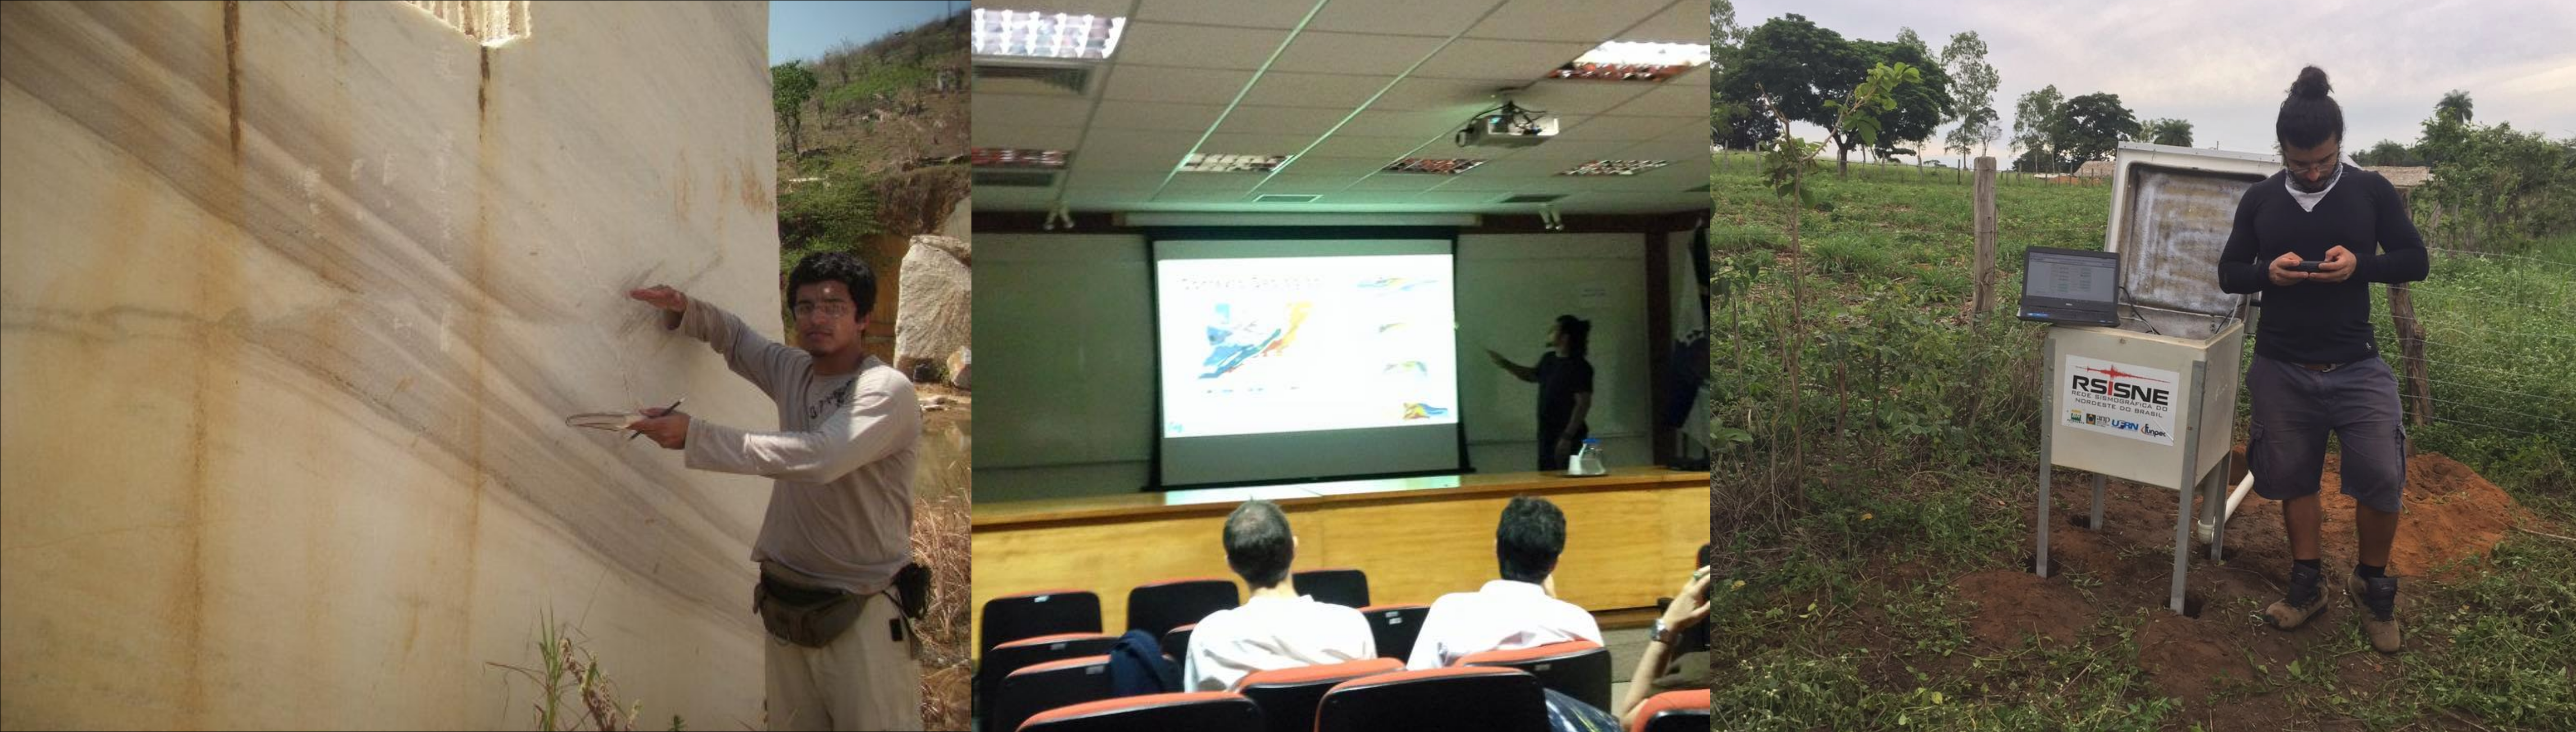
\includegraphics[width=\textwidth]{images/formacao.png}
  \end{center}
  \caption{
    Mosaico mostrando as diferentes fases da minha formação acadêmica. Esquerda: Realizando medidas estruturais no campo do trabalho de conclusão de curso na Serra de Itaóca Pedra-ES (2011). Centro: Apresentação do seminário dos estudantes no Observatório Nacional (2014). Instalação da estação sismográfica temporária na Bacia do Parnaíba (Maranhão) com o corpo técnico do \href{https://labsis.ufrn.br/}{LabSis-UFRN} (2017).
  }
 \label{fig_formacao}
\end{figure}

\begin{summarybox}[frametitle=\faAward{}\quad Resumo da formação acadêmica]
  \begin{datelist}
    2007--2012 & Bacharelado em Geologia -- Universidade Federal do Espírito Santo \\
    2013--2015 & Mestrado em Geofísica -- Observatório Nacional \\
    2015--2019 & Doutorado em Geodinâmica e Geofísica -- Universidade Federal do Rio Grande do Norte
  \end{datelist}
\end{summarybox}

Este capítulo relata a minha trajetória acadêmica, da Graduação ao Doutorado, explorando alguns detalhes que foram cruciais na construção da minha carreira e nos ajustes feitos durante o percurso.

\section{Universidade Federal do Espírito Santo}
\label{sec_ufrn}

\begin{subsummarybox}[frametitle=\faGraduationCap\quad Bacharelado em Geologia]
  \begin{fa-ul}
    \faFortAwesome & \textbf{Local:} Universidade Federal do Espírito Santo (Alegre-ES)\\
    \faClock & \textbf{Período:} Agosto 2007 -- Setembro 2012 \\
    \faUserTie & \textbf{Orientador:} Roberto Sacks de Campos\\
    \faChalkboardTeacher & \textbf{Tema:} Caracterização Estrutural e Petrológica dos Escarnitos da Região de Itaóca Pedra - ES.
  \end{fa-ul}
\end{subsummarybox}


Depois de algumas tentativas frustadas no vestibular do primeiro semestre de 2007, ingressei no curso de \href{https://geologia.ufes.br/}{Geologia} da \href{https://www.ufes.br/}{Universidade Federal do Espírito Santo} no segundo semestre. A combinação foi perfeita, já que o curso era na cidade de \href{https://alegre.es.gov.br/}{Alegre}, município do sul capixaba com uma população estimada de 30.000 habitantes, portanto era uma cidade próxima à minha cidade natal, pacata, segura e com um custo de vida baixo, ideal para um universitário.

\subsection{Conteúdo básico: Ciências Exatas}
\label{sec_geo_basico}

Eu tive uma boa aderência ao conteúdo programático do curso, tanto nas disciplinas específicas da Geologia, como nas disciplinas básicas (e.g., Cálculo, Física, Geometria analítica, Físico-química I), mesmo com grandes deficiências em tópicos básicos de física, resultado de problemas crônicos no ensino médio das escolas públicas brasileiras. Seguindo o conselho do saudoso professor de Cálculo I e II, \href{http://lattes.cnpq.br/8391815843000996}{Carlos Alberto Manfre}, decidi adicionar as disciplinas optativas de Cálculo III (ENG05506) e de Física III (ENG06034) para aprimorar meus conhecimentos na área. A última, ministrada pelo professor \href{http://lattes.cnpq.br/6503578618806955}{Roberto Colistete Júnior}, me impulsinou a estudar por conta própria a ligação da física com a geologia. No semestre seguinte, todo o conhecimento foi reforçado pela excelente disciplina de Geofísica Básica (ENG06501) ministrada pelo professor \href{http://lattes.cnpq.br/0799322864183147}{Welitom Rodrigues Borges}, fundamental para a minha escolha de seguir o estudo da Geofísica na pós-graduação. Um demonstrativo da melhora da minha base nas ciências exatas foi o convite para ser monitor da disciplina Físico-Química I (ENG05264) sob o comando da professora \href{http://lattes.cnpq.br/9146731989810239}{Raquel Vieira de Carvalho}.

\subsection{Conteúdo específico: Ciências Geológicas}
\label{sec_geo_especifico}

Na segunda parte do curso, resolvi adicionar tópicos relacionados a tecnologia após receber o convite da professora e amiga \href{http://lattes.cnpq.br/9513837515797451}{Fabricia Benda de Oliveira} para participar como colaborador voluntário do projeto \textbf{Identificação e mapeamento de áreas de risco geológico no município de Alegre-ES} e para ser monitor voluntário da parte computacional da disciplina de Mapeamento Geológico II (ENG06599). Devido a isso, adicionei várias disciplinas optativas relacionadas a \href{https://www.gov.br/economia/pt-br/assuntos/patrimonio-da-uniao/arquivos-anteriores-privados/programa-de-modernizacao/linha-do-tempo/34-sig-apostila.pdf}{Sistema de Informação Geográfica}, como Cartografia Temática e Digital (ENG06786), Análise e Modelagem Espacial  (ENG06867) e Sistemas Globais de Geoposicionamento (ENG06945). O curso me forneceu a oportunidade de conhecer as regiões Sul, Sudeste, Centro-Oeste e Nordeste do Brasil em diversas aulas de campo. A excepcional junção da base teórica sólida com essa experiência prática foi extremamente inspiradora para a minha formação como geocientista. Após trocar experiências vividas na UFES com alunos de outras instituições consagradas da Geologia, eu vi o esforço herculiano dos meus professores para nos proporcionarem uma base teórica sólida e aulas de campo nos  mais diversos contextos geológicos do Brasil. Essa é uma tarefa desafiadora para um curso recente, especialmente vinculado a um campus localizado em uma região interiorana de um pequeno estado brasileiro. Até hoje continuo utilizando os conceitos que aprendi nas disciplinas do ciclo profissionalizante, como a excelente disciplina de Geologia Estrutural (ENG06600) ministrada pelo professor \href{http://lattes.cnpq.br/1004206862799097}{Fernando Jacques Althoff} e Geologia do Brasil pelo professor \href{http://lattes.cnpq.br/5883057974133630}{Felipe Guadagnin}. Durante o trabalho de conclusão de curso (TCC) utilizei os conceitos de todas essas disciplinas, como também das disciplinas proferidas pelo meu orientador \href{http://lattes.cnpq.br/5081674111092263}{Roberto Sacks de Campos}, como Geoquímica (ENG06506) e Petrologia Metamórfica (ENG06865). A elaboração do TCC, entitulado \href{https://doi.org/10.6084/m9.figshare.25366483.v1}{Caracterização Estrutural e Petrológica dos Escarnitos da Região de Itaóca Pedra - ES}, foi uma experiência muito enriquecedora, pois organizei as viagens de campo, a preparação das lâminas e todo o calendário de execução das etapas de forma independente. Todo esse trabalho foi crucial para compreender que o processo de concepção e implementação de um projeto é um empreendimento extenso e requer dedicação intensa.

\subsection{Bolsa de Pesquisa (2011-2012)}
\label{sec_bolsa_hidro}

\begin{summarybox}[frametitle=\faProjectDiagram{}\quad Resumo do projeto]
  \begin{datelist}
    \faFile* & Levantamento Hidrogeológico do Estado do Espírito Santo \\
    \faHammer & Universidade Federal do Espírito Santo e Universidade Federal do Ceará \\
    \faCalendar*[regular] & 24 meses \\
    \faMapMarked* & 37 municípios dos Espírito Santo \\
    \faUserTie & Paulo de Tarso Ferro de Oliveira Fortes \\
    \faWallet & Petrobras \\
    \faMoneyBill*[regular] & R\$ 3.447.638,38
  \end{datelist}
\end{summarybox}

No segundo semestre de 2011, durante meu último ano de graduação, fui aprovado no processo seletivo para bolsista no projeto de Pesquisa \& Desenvolvimento \href{https://contratos.ufes.br/sites/contratoseconvenios.ufes.br/files/field/anexo/projeto_basico462015.pdf}{Levantamento Hidrogeológico do Estado do Espírito Santo}, desenvolvido em conjunto pela Universidade Federal do Espírito Santo e pela Universidade Federal do Ceará e coordenado pelo professor \href{http://lattes.cnpq.br/5417271870207313}{Paulo de Tarso Ferro de Oliveira Fortes}. Tal projeto tinha a finalidade de caracterizar regionalmente o potencial hídrico dos aquíferos e reservatórios rasos das províncias sedimentares e cristalinas, localizadas em 37 municípios no estado do Espírito Santo, visando a explotação racional destes recursos para sua utilização em usos diversificados. O projeto foi executado com recursos financeiros da Petrobras, onde eu recebia uma bolsa através da \href{https://mapaosc.ipea.gov.br/detalhar/1246897}{Fundação Ceciliano Abel de Almeida (FCAA)} para executar os seguintes objetivos:

\begin{itemize}
  \item Organização da base cartográfica digital das folhas topográficas Linhares, Rio Doce, Baixo Guandu, Colatina, Montanha e Nanuque (IBGE - 1:100.000);
  \item Desenvolvimento de atividades de campo no período de 13 a 18/02/2012 visando o cadastramento de poços tubulares profundos.
\end{itemize}

A participação neste projeto foi um marco na minha trajetória acadêmica, pois aprendi a trabalhar de maneira síncrona com uma grande equipe de alunos. A experiência me proporcionou a chance única de explorar o interior da região norte do Espírito Santo, conhecendo de um outro ângulo as características culturais e geográficas locais. Ao testemunhar de perto a execução de um projeto de grande envergadura, fui capaz de absorver valiosos ensinamentos e aprender na prática, aprimorando assim minha compreensão sobre a implementação eficaz de iniciativas desse porte.

\subsection{Bolsa de Estágio (2012)}
\label{sec_bolsa_petro}

\begin{summarybox}[frametitle=\faInfoCircle{}\quad Resumo do estágio]
  \begin{datelist}
    \faFile* & Estágio Supervisionado em Geologia \\
    \faCalendar*[regular] & 3 meses (Junho a Agosto) \\
    \faMapMarked* & E\&P-SERV/US-SUB/GM (Geologia Marinha/Macaé-RJ) \\
    \faUserTie & Marco Aurélio de Campos Merschmann \\
    \faWallet & Petrobras
  \end{datelist}
\end{summarybox}

No final do primeiro semestre de 2012, fui selecionado no processo seletivo para estagiário na Unidade de Serviços Submarinos da \href{https://petrobras.com.br/}{Petrobras}, mais precisamente na gerência de Geologia Marinha, que na época era chefiada pelo geofísico \href{https://br.linkedin.com/in/marco-aur\%C3\%A9lio-merschmann-b9381823}{Marco Aurélio de Campos Merschmann}. O estágio foi realizado na Petrobras S.A., localizada no município de Macaé, no estado do Rio de Janeiro. O plano de trabalho englobava atividades nas bases de Imboassica, setor de Geologia Marinha, e Imbetiba, laboratório de Sedimentologia e Estratigrafia. Os objetivos propostos para o estágio foram:

\begin{itemize}
  \item Acompanhamento de mapeamento de dados sísmicos 3D e  de alta freqüência;
  \item Acompanhamento da descrição de testemunhos geológicos (Laboratório de Sedimentologia);
  \item Acompanhamento da elaboração de laudos para subsidiar a perfuração de poços, instalação de equipamentos submarinos e dutos;
  \item Leitura e análise de conteúdo dos relatórios de estudos de \href{https://en.wikipedia.org/wiki/Geological_hazard}{geohazard}.
\end{itemize}

A primeira dificuldade encontrada foi na sistemática corporativa empregada pela Petrobras, principalmente no grande número de siglas e equipamentos utilizados. No entanto, a partir do estudo dos laudos técnicos e de esclarecimentos pontuais por parte da equipe de técnicos, a adaptação evoluiu em um ritmo acelerado. Este estágio foi muito proveitoso para entender o funcionamento de uma grande empresa do setor energético, principalmente conhecer as rotinas de trabalho utilizadas pelos técnicos da Geologia Marinha para armazenar, carregar, modelar, calcular e converter dados geológicos e geofísicos. Outro trabalho que foi um diferencial nesse estágio foi a abertura, descrição, documentação, datação e interpretação de testemunhos geológicos. Vale destacar que graças à disciplina optativa Geologia do Quaternário (ENG05572), ministrada pelo professor \href{http://lattes.cnpq.br/6157185791642499}{Cláudio Eduardo Lana}, pude acompanhar sem problemas o trabalho no Laboratório de Sedimentologia, o que não era comum, pois é uma área muito específica nas ciências geológicas.

Avaliando todos os pontos vivenciados durante este período, tanto positivos quanto negativos, posso atestar que essa experiência foi bastante proveitosa na minha carreira, englobando experiências no campo relacional (gestão de pessoas) e no campo intelectual (contato direto com o estado da arte na tecnologia do setor de petrolífero).

\section{Observatório Nacional}
\label{sec_on}

\begin{subsummarybox}[frametitle=\faGraduationCap{}\quad Mestrado em Geofísica]
  \begin{fa-ul}
    \faFortAwesome & \textbf{Local:} Observatório Nacional (Rio de Janeiro-RJ) \\
    \faClock & \textbf{Período:} Março 2013 -- Abril 2015 \\
    \faUserTie & \textbf{Orientador:} Stéphane Gérard Martial Drouet\\
    \faUserTie & \textbf{Coorientador:} Bruno Yann Nicolas Goutorbe\\
    \faWallet & \textbf{Bolsista:} Conselho Nacional de Desenvolvimento Científico e Tecnológico - CNPQ \\
    \faChalkboardTeacher & \textbf{Tema:} Análise da Estrutura Crustal na Faixa Ribeira (entre as Províncias do Cráton São Francisco e da Bacia do Paraná) utilizando Métodos Sismológicos.
  \end{fa-ul}
\end{subsummarybox}

Ainda no estágio, conversando com os geólogos e geofísicos da gerência de Geologia Marinha, fui alertado sobre as vantagens de continuar os estudos e entrar em uma instituição de pesquisa científica. Observando o benefício da exposição a uma diversidade de formas de pensamento oriunda de diferentes locais e instituições, decidi que estava na hora de mudar minha realidade, indo para uma metrópole e uma instituição de pesquisa consagrada no Brasil. Devido a fatores logísticos e operacionais, o \href{https://www.gov.br/observatorio/pt-br}{Observatório Nacional (ON)} despertou meu interesse. No final de 2012 prestei concurso para o \href{https://www.gov.br/observatorio/pt-br/assuntos/programas-academicos/pos-graduacao-em-geofisica}{Programa de Pós-graduação em Geofísica do ON} e no começo de março de 2013 iniciei os estudos. Mesmo não tendo um orientador e um projeto no início do mestrado, eu estava convencido que trabalharia com algum tema relacionado a Terra Sólida. Após algumas tratativas, iniciei o projeto de mestrado com o professor \href{http://lattes.cnpq.br/0563544084744404}{Stéphane Gérard Martial Drouet} com dados de estações sismográficas temporárias de banda larga instaladas no Sudeste do Brasil.

\subsection{Ambiente da Pós-graduação}
\label{sec_posgrad_on}

O ambiente da pós-graduação do ON era extremamente diverso e cientificamente estimulante, pois as salas mesclavam doutorandos e mestrandos de diversas áreas da geofísica e astronomia. A multiculturalidade era gigantesca. Devido a isso, o ambiente era acolhedor e as conversas informais eram cheias de conselhos. Essas dicas informais foram fundamentais para o meu crescimento como cientista. Como eu sou oriundo da Geologia, eu tinha muita experiência prática nas Geociências, no entanto, eu tinha uma conhecimento teórico muito raso. Graças às conversas com os físicos, geólogos e geofísicos, tantos que seria indelicado tentar citar neste texto, eu iniciei os estudos de inversão e programação em \href{https://www.python.org/}{python}. Além disso, recebi inúmeros conselhos e dicas para um processamento correto dos dados nas disciplinas de Inversão Linear em Geofísica (INVL) e Problemas Inversos em Geofísica (PIGEO), ministradas pelos professores \href{http://lattes.cnpq.br/4332841435949533}{Vanderlei Coelho de Oliveira Junior} e \href{http://lattes.cnpq.br/0391036221142471}{Valéria Cristina Ferreira Barbosa}. Somado a isso, fui incentivado a retrabalhar os dados oriundos do meu trabalho de conclusão de curso utilizando métodos aeromagnetométricos e aeroradiométricos para correlacionar com o mapeamento geológico realizado. Com isso, no primeiro semestre do mestrado eu publiquei um resumo expandido, entitulado \href{https://doi.org/10.1190/sbgf2013-129}{Aerogeophysical data to refine geological mapping: A semi-quantitative approach}, no 13th Congresso Internacional da Sociedade Brasileira de Geofísica entre 26 e 29 de Agosto 2013. Mesmo não pertecendo a nenhum projeto grande, o PPG-ON me forneceu a oportunidade de frequentar congressos nacionais e internacionais, onde pude corrigir minhas pendências na pesquisa científica.

\subsection{Projeto de Mestrado}
\label{sec_proj_mest}

Meu projeto de mestrado, sob a orientação do professor Stéphane Drouet, era a análise e delimitação de grandes feições estruturais crustais através dos resultados de duas metodologias distintas: Função do Receptor de onda P e Tomografia de Ruído Sísmico Ambiental (momento em que o professor \href{http://lattes.cnpq.br/5754348793953158}{Bruno Yann Nicolas Goutorbe} entrou como co-orientador no mestrado). Os dados eram oriundos de estações temporárias do projeto \href{http://www.pegbr.on.br:8080/pegbr/visualizar/SolicitacaoDadosProjeto.jsp?cod=74}{SUBSAL} e estações permanentes da \href{www.rsbr.on.br}{Rede Sismográfica Brasileira}. Os resultados oriundos das Funções do Receptor foram apresentadados em um resumo expandido, entitulado \href{http://dx.doi.org/10.22564/6simbgf2014.043}{Analysis of Crustal Structure in the region of Ribeira Belt (between the Provinces of the São Francisco Craton and the Paraná Basin) using Seismological Methods}, enviado para o VI Simpósio Brasileiro de Geofísica entre 14 e 16 de Outubro de 2014. Devido à excelente colaboração, o professor Bruno Goutorbe me convidou para colaborar na interpretação dos resultados provenientes da Tomografia de Ruído obtidos a partir de 53 estações sismográficas permanentes espalhadas pelo território brasileiro no período de 1996 a 2012. O trabalho entitulado \href{http://dx.doi.org/10.1093/gji/ggv343}{Rayleigh wave group velocities at periods of 6-23 s across Brazil from ambient noise tomography} foi publicado no segundo semestre de 2015. Terminei meu mestrado em abril de 2015 e iniciei o processo de entrada no Doutorado em Geofísica do Observatório Nacional, no entanto, por ironia do destino, os meus orientadores não permaneceram no Brasil e eu tive que reajustar a direção da minha carreira.

\bigskip

\begin{summarybox}[frametitle=\faBookmark{}\quad Resumo de atividades científicas]
	\begin{fa-ul}
		\faBook & Resumo Expandido (2013): 13th International Congress of the Brazilian Geophysical Society \& EXPOGEF. \href{https://doi.org/10.1190/sbgf2013-129}{Aerogeophysical data to refine geological mapping: A semi-quantitative approach}. \textbf{Diogo Luiz de Oliveira Coelho} e Felipe Guadagnin. \\
		\faBook & Resumo Expandido (2014): VI Simpósio Brasileiro de Geofísica. \href{http://dx.doi.org/10.22564/6simbgf2014.043}{Analysis of Crustal Structure in the region of Ribeira Belt (between the Provinces of the São Francisco Craton and the Paraná Basin) using Seismological Methods}. \textbf{Diogo Luiz de Oliveira Coelho} e Stéphane Drouet. \\
		\faBook & Artigo publicado (2015): Geophysical Journal International. \href{http://dx.doi.org/10.1093/gji/ggv343}{Rayleigh wave group velocities at periods of 6-23s across Brazil from ambient noise tomography}. Bruno Goutorbe, \textbf{Diogo Luiz de Oliveira Coelho}, Stéphane Drouet. 
	\end{fa-ul}
\end{summarybox}

\section{Universidade Federal do Rio Grande do Norte}
\label{sec_doutorado}

\begin{subsummarybox}[frametitle=\faGraduationCap{}\quad Doutorado em Geodinâmica e Geofísica]
  \begin{fa-ul}
    \faFortAwesome & \textbf{Local:} Universidade Federal do Rio Grande do Norte  (Natal-RN)  \\
    \faClock & \textbf{Período:} Agosto 2015 -- Dezembro 2019 \\
    \faUserTie & \textbf{Orientador:} Jordi Julià Casas \\
    \faWallet & \textbf{Bolsista:} Fundação Norte-Rio-Grandense de Pesquisa e Cultura - FUNPEC \\
    \faChalkboardTeacher & \textbf{Tema:} Sismologia de fonte passiva na bacia do Parnaíba: Implicações para a subsidência cratônica.
  \end{fa-ul}
\end{subsummarybox}

\begin{summarybox}[frametitle=\faProjectDiagram{}\quad Resumo do projeto]
  \begin{datelist}
    \faFile* & Parnaíba Basin Analysis Project (PBAP) \\
    \faHammer & Universidade Federal do Rio Grande do Norte  e Universidade de Cambridge \\
    \faCalendar*[regular] & 2012 - 2017 \\
    \faMapMarked* & Bacia do Parnaíba \\
    \faUserTie & Jordi Julià Casas \\
    \faWallet & BP Energy do Brasil LTDA  \\
    \faMoneyBill*[regular] & R\$ 1.998.038,98
  \end{datelist}
\end{summarybox}

Após a finalizar o mestrado e ser notificado que não teria mais a possibilidade de continuar como aluno da área de Sismologia no Obseratório Nacional, optei por mudar de instituição para me manter na área e aprimorar os meus estudos em tópicos relacionados à Sismologia. No mestrado eu tive uma formação sólida como geofísico, no entanto, carecia de estudos profundos em tópicos específicos da Sismologia. Conversando com professores, recebi uma notificação que abrira uma vaga para doutorado no \href{https://posgraduacao.ufrn.br/325}{Programa de Pós-Graduação em Geodinâmica e Geofísica} da UFRN na área de Sismologia com o professor \href{http://lattes.cnpq.br/0012168139768170}{Jordi Julià Casas}. Conversando novamente com familiares e amigos, decidi que seria interessante viver uma nova experiência no Nordeste do Brasil. Com isso, em agosto de 2015, me mudei para Natal-RN, para novamente mudar minha realidade, indo para uma cidade localizada no extremo nordeste do país. Realmente, foi uma decisão acertada, pois a cidade é uma capital com cara de interior, onde o sol brilha o ano todo. 

\subsection{Projeto de Doutorado}
\label{sec_proj_doc}

Meu projeto de Doutorado foi financiado pelo PBAP, sendo um braço na busca da caracterização estrutural profunda da \href{https://www.gov.br/anp/pt-br/rodadas-anp/rodadas-concluidas/concessao-de-blocos-exploratorios/14a-rodada-licitacoes-blocos/arquivos/areas-oferta/sumario-parnaiba.pdf}{Bacia do Parnaíba} através da sísmica passiva. As metodologias utilizadas, inversão conjunta e migração pré-empilhamento, tiveram a finalidade de expor as principais descontinuidades sísmicas na crosta e no manto para elucidar como o arcabouço geológico se comportou em meio aos processos geológicos que atuaram abaixo da bacia. No primeiro ano do doutorado eu me dediquei aos estudos das diversas disciplinas envolvendo tópicos da Sismologia. Além disso, como mostrado na Figura \ref{fig_formacao}, no primeiro ano do Doutorado eu me dediquei à implantação do perfil de estações sismográficas temporárias na Bacia do Parnaíba, sendo que a última estação instalada estava localizada a aproximadamente 2000 km de distância de Natal-RN. Todo este percurso foi realizado em seguidas viagens de carro, onde pude vivenciar todo o trabalho realizado pelos técnicos do LabSis-UFRN para manter em funcionamento a \href{https://labsis.ufrn.br/}{Rede Sismográfica do Nordeste (RSISNE)}. As longas viagens foram proveitosas para também criar um vínculo com os técnicos do laboratório, principalmente com \href{http://lattes.cnpq.br/0406798380417692}{Eduardo Alexandre Santos de Menezes}, quando em uma conversa sobre uma boa metodologia para atestar a qualidade de uma estação sísmográfica, confeccionamos o trabalho \href{https://dx.doi.org/10.6084/m9.figshare.25367143}{Assessing data quality and station performance for eight meridian compact posthole stations deployed in the parnaíba basin}, que foi apresentado no II Simpósio Brasileiro de Sismologia entre 12 a 15 de novembro de 2017. Este trabalho gerou um conjunto de códigos\footnote{Python framework for analysing the quality of seismological data archived in based on ObsPy em \url{https://github.com/dIOGOLOC/codes_escritos/tree/b0f5c54cf46a37c2642732c47bcb422bf00495fd/LabSis_controle_de_qualidade}} que o LabSis utiliza para o controle de qualidade dos seus equipamentos.  

Os resultados da tese apresentaram metodologias diferentes para caracterizar a estrutura crustal e da parte mais rasa do manto superior abaixo da Bacia do Parnaíba e para imagear a Zona de Transição do Manto (limite entre o manto superior e o manto inferior). Na primeira parte, os métodos utilizados estimaram pontualmente a espessura da crosta e a razão Vp/Vs nas estações sismográficas de banda larga sobre a bacia. Juntamente com essas estimativas foram recuperados perfis de velocidade da onda S em função da profundidade através de uma inversão conjunta de dados sismológicos. Os resultados desses estudos foram bem relevantes e foram apresentados em conferências nacionais\footnote{Anais do 48 Congresso Brasileiro de Geologia, 2016, Porto Alegre em \url{http://cbg2017anais.siteoficial.ws/ste01/ID5293_110479_52_48CBG_Diogo.pdf}} e internacionais\footnote{19th EGU General Assembly, EGU2017, proceedings from the conference held 23-28 April, 2017 in Vienna, Austria., p.10252 em \url{https://ui.adsabs.harvard.edu/abs/2017EGUGA..1910252C/abstract}}. Estes resultados estavam em sintonia com outros métodos geofísicos realizados sobre o mesmo perfil, então, no primeiro semestre de 2018, o primeiro artigo do doutorado foi publicado com o título \href{https://doi.org/10.1144/SP472.8}{Deep crustal architecture of the Parnaíba basin of NE Brazil from receiver function analysis: implications for basin subsidence}.

\subsection{Eventos Marcantes no Doutorado}
\label{sec_ev_doc}

Dois eventos foram muito marcantes no meu doutorado, o primeiro foi em meados de 2016, onde participei da \href{https://indico.ictp.it/event/7615/material/11/0.jpg}{School on Seismology beyond Textbooks} entre 29 de Agosto e 3 Setembro de 2016 no Centro Internacional de Física Teórica em Trieste-IT. Nesta escola eu pude ter um encontro com diversos doutorandos ao redor do mundo, além de interagir com grandes cientistas na área da Sismologia Moderna, como é o exemplo do professor \href{https://scholar.google.fr/citations?user=ZCRP01AAAAAJ&hl=fr}{Michel Campillo}, do qual eu utilizei a metodologia para fazer os trabalhos sobre Tomografia de Ruído Sísmico. O segundo evento marcante foi em meados de 2017, o \href{https://geodynamics.org/events/details/218}{CIG-LLNL Computational Seismology Workshop} no Laboratório Nacional Lawrence Livermore na Califórnia. O objetivo do workshop foi fornecer aos participantes uma experiência prática no acesso, processamento, modelagem e visualização de dados sísmicos usando ferramentas avançadas em Sismologia em um supercomputador. A partir dessas experiências, retornei a Natal-RN com o pensamento de aprimorar as minhas rotinas de programação criadas durante o processamento de dados. 

A partir do segundo ano de doutorado, iniciei o processo que mudou a minha formação: criar um pacote de códigos estruturados e de fácil reprodutibilidade para toda metodologia que eu fosse utilizar. Com isso, iniciei os estudos sobre a Zona de Transição do Manto e sobre o processo de migração das Funções do Receptor. Após um longo período estudando e programando, eu criei um pacote computacional\footnote{Python framework for receiver functions migration em \url{https://github.com/dIOGOLOC/codes_escritos/tree/b0f5c54cf46a37c2642732c47bcb422bf00495fd/mantle_transition_zone_migration_obspy_Pds}} que migra as formas de onda de tempo para profundidade. Com os resultados encontrados, eu consegui avaliar o papel dos processos convectivos profundos e das heterogeneidades do manto na formação e evolução da Bacia do Parnaíba. Novamente foi um salto muito grande na minha caminhada acadêmica investigar as descontinuidades mantélicas, pois é natural para um geólogo entender a estrutura da Crosta da Terra porque é visível, porém o arcabouço do Manto estava totalmente fora da minha zona de conforto. Nossos resultados mostraram que a espessura da zona de transição se mantém constante sob a bacia, isto é, não existe nenhuma evidência nesta camada de um fluxo vertical negativo pretérito ou heterogeneidade mantélica que possa ter influenciado no processo de formação da bacia. O artigo entitulado \textit{"Mantle transition zone topography beneath the Parnaíba basin of NE Brazil: New constraints on deep mantle dynamics"} foi submetido em 2019 à revista Geophysical Journal International e obteve um parecer positivo para publicação após correções relativamente pequenas. No entanto, devido a problemas de cunho pessoal e situações da pandemia que se iniciou no começo de 2020, eu não continuei com a submissão. Creio que foi uma decisão acertada, pois estou reformulando novamente o artigo. Atualizando o banco de dados para 2024, agora tenho resultados e discussões mais sólidas.

\bigskip

\begin{summarybox}[frametitle=\faBookmark{}\quad Resumo de atividades científicas]
	\begin{fa-ul}
		\faBook & Resumo (2016): 48 Congresso Brasileiro de Geologia. \href{http://cbg2017anais.siteoficial.ws/ste01/ID5293_110479_52_48CBG_Diogo.pdf}{Characterizing the Lithospheric Architecture of the Parnaíba Basin with Passive-Source Seismology}. \textbf{Diogo Luiz de Oliveira Coelho} e Jordi Juliá. \\
		\faBook & Resumo (2017): 19th EGU General Assembly 2017. \href{https://meetingorganizer.copernicus.org/EGU2017/EGU2017-10252.pdf}{Characterizing the Crustal architecture of the Parnaiba basin with passive-source seismology}. \textbf{Diogo L. O. Coelho}, Jordi Julià, Verónica Rodríguez-Tribaldos e Nicholas White. \\
		\faBook & Resumo (2017): 19th EGU General Assembly 2017. \href{https://meetingorganizer.copernicus.org/EGU2017/EGU2017-9897.pdf}{Deep Structure and Subsidence History of Parnaíba Cratonic Basin, NE Brazil}. Verónica Rodríguez Tribaldos, Nicky J. White, \textbf{Diogo Luiz de Oliveira Coelho} e Jordi Julià. \\
		\faBook & Resumo (2017): II Simpósio Brasileiro de Sismologia. \href{https://dx.doi.org/10.6084/m9.figshare.25367143}{Assessing data quality and station performance for eight meridian compact posthole stations deployed in the Parnaíba Basin}. \textbf{Diogo Luiz de Oliveira Coelho}, Eduardo Alexandre Santos de Menezes e Jordi Julià \\
		\faBook & Artigo publicado (2018): Geological Society, London, Special Publications. \href{https://doi.org/10.1144/sp472.8}{Deep crustal architecture of the Parnaíba basin of NE Brazil from receiver function analysis: implications for basin subsidence}. \textbf{Diogo L. O. Coelho}, Jordi Julià, Verónica Rodríguez-Tribaldos e Nicholas White. \\
		\faBook & Artigo em finalização (2024): Nossos resultados revelam uma espessura média de MTZ de 252$\pm$7,5 km sob esta bacia, semelhante ao valor nominal de 250 km dos modelos globais, com variações entre 232 e 279 km.. Mantle transition zone topography beneath the Parnaíba basin of NE Brazil: New constraints on deep mantle dynamics. \textbf{Diogo L. O. Coelho}, Jordi Julià, Verónica Rodríguez-Tribaldos e Nicholas White. 
	\end{fa-ul}
\end{summarybox}

%==============================================================================
\chapter{Atuação Profissional}
\label{cap_atuacao}

\begin{figure}[h]
  \HeroFigPad
  \begin{center}
    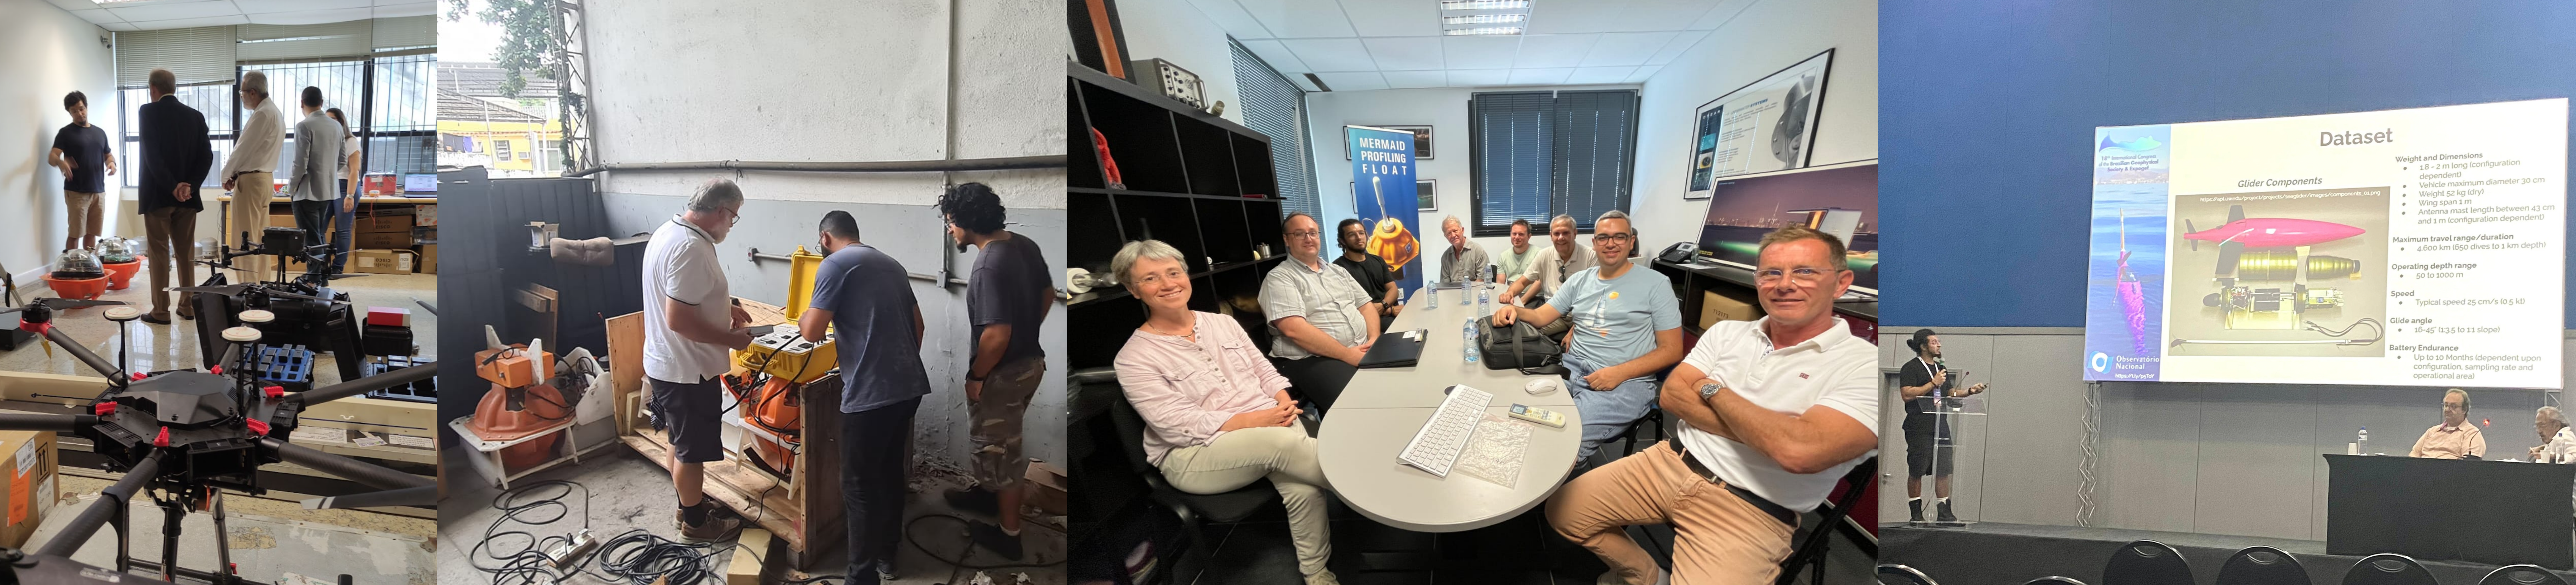
\includegraphics[width=\textwidth]{images/atuacao_pos.png}
  \end{center}
  \caption{
    Mosaico mostrando as diversas frentes de atuação durante o período do estágio pós-doutoral no Observatório Nacional. Primeira: Recebendo e apresentando os equipamentos utilizados nas campanhas de aquisição de dados no fundo oceânico à Diretoria de Desenvolvimento Científico e Tecnológico da \href{http://www.finep.gov.br/}{FINEP} (2024). Segunda: Recebendo o engenheiro da \href{https://www.guralp.com/}{Güralp} para a manuntenção dos Sismômetros de Fundo Oceânico (2022). Terceira: Representante da comitiva da RSBR na empresa francesa \href{https://www.linkedin.com/company/osean-sas}{OSEAN} para aquisição dos Sismógrafos flutuantes (\href{https://www.geoazur.fr/GLOBALSEIS/Mermaid.html}{MERMAID} - 2023). Quarta: Apresentação de trabalho científico no \href{https://sbgf.org.br/congresso/}{18th International Congress of the Brazilian Geophyisical Society and EXPOGEf} (2023).}
\end{figure}
    
\bigskip

\begin{summarybox}[frametitle=\faInfoCircle{}\quad Resumo da atuação profissional]
  \begin{datelist}
    2020--2021 & Estágio Pós-doutoral I -- Universidade Federal de Santa Catarina \\
    2022--2023 & Estágio Pós-doutoral II -- Observatório Nacional \\
    2023--atual & Estágio Pós-doutoral III -- Observatório Nacional \\
  \end{datelist}
\end{summarybox}

\bigskip

Este capítulo relata minha atuação profissional e as seções abaixo se referem às atividades institucionais e experiências pessoais nesta caminhada (seções \ref{sec_posdoc_ufsc},\ref{sec_posdoc_pci} e \ref{sec_posdoc_glider}). Já as atividades relacionadas à divulgação científica, formação de capital humano e atividades de ensino serão descritas nos capítulos \ref{cap_ensino} e \ref{cap_comunidade}, respectivamente. Durante meu estágio pós-doutoral, concentrei meus esforços em explorar novas fronteiras do conhecimento sismológico e desenvolver pesquisas e tecnologias inovadoras contribuindo para avanços significativos na Sismologia Marinha, uma área de estudo que abracei no início de 2020. Além disso, dediquei parte do meu tempo orientando estudantes de iniciação científica e participando da pós-graduação do Observatório Nacional, através da ministração de aulas, participação em bancas e coordenação do \href{https://www.gov.br/observatorio/pt-br/assuntos/programas-academicos/pos-graduacao-em-geofisica/seminarios}{Ciclo de Seminário do Programa de Pós-graduação em Geofísica}. Adicionalmente, fui voluntário em atividades de divulgação e popularização da ciência junto à \href{https://www.gov.br/observatorio/pt-br/assuntos/areas-de-atuacao/divulgacao-e-popularizacao-da-ciencia}{Divisão de Comunicação e Popularização da Ciência}, onde busquei ativamente estreitar os laços entre a instituição e a sociedade. Participei de eventos, palestras e de entrevistas, onde esclareci dúvidas da sociedade em tópicos relacionados à Sismologia e Tectônica. Ao longo dessas experiências institucionais e pessoais, obtive um crescimento vertiginoso, tanto intelectualmente como profissionalmente, e pude perceber o grande impacto na minha carreira acadêmica neste estágio pós-doutoral no Observatório Nacional.

\section{Universidade Federal de Santa Catarina (2020-2021)}
\label{sec_posdoc_ufsc}

\begin{subsummarybox}[frametitle=\faUniversity{}\quad Vínculo institucional]
  \begin{fa-ul}
    \faUser & Estágio pós-doutoral \\
    \faMapMarker & Programa de Pós-Graduação em Oceanografia (UFSC)\\
    \faCalendar & Março 2020 -- Novembro 2021
  \end{fa-ul}
\end{subsummarybox}

\begin{summarybox}[frametitle=\faProjectDiagram{}\quad Resumo do projeto]
  \begin{datelist}
    \faFile* & Monitoramento Sismológico e Oceanográfico de um Segmento na Margem Sudeste do Brasil: Norte da Bacia de Santos ao Sul da Bacia do Espírito Santo \\
    \faHammer & Universidade Federal de Santa Catarina e Observatório Nacional \\
    \faCalendar*[regular] & 2017 - 2022 \\
    \faMapMarked* & Margem Sudeste do Brasil \\
    \faUserTie & Antonio Henrique da Fontoura Klein \\
    \faWallet & Petrobras  \\
    \faMoneyBill*[regular] & R\$ 7.469.026,31
  \end{datelist}
\end{summarybox}

Esta seção relata a experiência que tive trabalhando no \href{https://sismo-oceano.ufsc.br/projeto-obs/}{Projeto Monitoramento Sismo-Oceanográfico}. Após a defesa de Doutorado, os professores \href{http://lattes.cnpq.br/8537150955145617}{Sergio Luiz Fontes} e \href{http://lattes.cnpq.br/2354029280846247}{Antonio Henrique da Fontoura Klein} me convidaram para participar do projeto dando enfoque ao processamento dos dados sismológicos coletados durante a campanha de aquisição. O projeto tinha como meta integrar atividades sismológicas, sismoestratigráficas e de variáveis oceanográficas para avançar no entendimento da geodinâmica da margem sudeste e ampliar o conhecimento e detecção de variáveis responsáveis por gerar deslizamentos de sedimentos do talude e, consequentemente, planejar ações da indústria do petróleo para implantação de infraestrutura de exploração e produção de hidrocarbonetos. Para cumprir esses objetivos foram instalados em 2019 seis Sismômetros de Fundo Oceânico (OBS) pertencentes ao \href{https://www.gov.br/observatorio/pt-br/servicos/servicos-geofisica/pool-de-equipamentos-geofisicos}{Pool de Equipamentos Geofísicos} do Observatório Nacional (ON) na Margem Sudeste do Brasil. Os dados coletados foram integrados às estações terrestres permanentes da \href{www.rsbr.gov.br}{Rede Sismográfica Brasileira}, as quais ampliaram para o mar a capacidade de monitoramento sísmico. Além disso, o projeto instalou um fundeio oceanográfico (1200m de profundidade) para coleta de dados de temperatura, salinidade e correntes, e realizou levantamentos hidrográficos e de sísmica rasa. Em 2020, mesmo com o agravamento da crise humanitária pela pandemia, os OBSs foram recuperados. Inicialmente, eu estaria no cruzeiro de recuperação dos equipamentos, no entanto, a tripulação teve que ser reduzida para evitar a contaminação. Então, infelizmente, não pude participar de nenhuma campanha de instalação e recuperação de equipamentos do projeto. Superadas as dificuldades operacionais, com os dados em mãos, as atividades do estágio pós-doutoral foram iniciadas para realizar os objetivos propostos no projeto.

Foi uma época muito complicada, pois enfrentar os desafios deste novo projeto isolado em minha casa foi uma tarefa repleta de aprendizado e superação. Um evento que me ajudou muito nesta etapa foi o \href{https://www.iris.edu/hq/workshops/2021/03/mss}{Marine Seismology Symposium}, que foi a minha única chance de observar outros resultados de campanhas com OBSs e assistir discussões sobre as direções futuras na Sismologia Marinha. Mesmo me deparando com uma área totalmente desconhecida, consegui superar os obstáculos e apresentar resultados bem promissores do processamento de dados no \href{https://sbgf.org.br/17th_cisbgf/}{17 Congresso Internacional da Sociedade Brasileira de Geofísica e EXPOGEf}. A imersão em uma área tão pouco explorada pela ciência sismológica exigiu um grande esforço para assimilar conceitos complexos e desenvolver metodologias para o processamento de dados tão ruidosos e em um contexto geológico tão diferente. Grande parte do desafio foi superado e as discussões ainda estão em finalização para a confecção do artigo: \textit{Seismicity, performance and noise recorded by ocean bottom seismometers monitoring of the Southeast Offshore of Brazil}. Essa jornada de descoberta e superação não apenas ampliou meus horizontes profissionais, mas também reforçou minha convicção na importância de mergulhar em novas áreas do conhecimento sismológico.

\bigskip

\begin{summarybox}[frametitle=\faBookmark{}\quad Resumo de atividades científicas]
	\begin{fa-ul}
		\faBook & Resumo (2021):  17 Congresso Internacional da Sociedade Brasileira de Geofísica e EXPOGEf. \href{https://sbgf.org.br/mysbgf/eventos/expanded_abstracts/17th_CISBGf/170620210624192518Expanded_abstract_SBGf_2021.pdf}{ New horizons in Brazilian Seismology: expanding seismic monitoring to offshore Southeast Brazil.}. \textbf{COELHO, D. L. O.}; FONTES, S. L.; KLEIN, A. H. F.; DIAS, F. L.; MAURICIO, I. C. B. S.; MACHADO, A. A.; PRADO, M. F. V.; LIMA, A. P. Y.; SILVA, A. A. C.; THEODORO, C.E.; ROSALBA, J. F.; SOBREIRA, J. F. F.; MAHIQUES, M. M.; BUENO, G. V. \\
\faBook & Artigo em finalização (2024): Resultados da análise do banco de dados coletado pelos sismômetros de fundo oceânico. Seismicity, performance and noise recorded by ocean bottom seismometers monitoring of the Southeast Offshore of Brazil. \textbf{COELHO, D. L. O.}; FONTES, S. L.; KLEIN, A. H. F.; DIAS, F. L.; MAURICIO, I. C. B. S.; MACHADO, A. A.; PRADO, M. F. V.; LIMA, A. P. Y.; SILVA, A. A. C.; THEODORO, C.E.; ROSALBA, J. F.; SOBREIRA, J. F. F.; MAHIQUES, M. M.; BUENO, G. V. 
	\end{fa-ul}
\end{summarybox}

\section{Observatório Nacional (2021-2023)}
\label{sec_posdoc_pci}

\begin{subsummarybox}[frametitle=\faUniversity{}\quad Vínculo institucional]
  \begin{fa-ul}
    \faUser & Estágio pós-doutoral \\
    \faMapMarker & Programa de Pós-Graduação em Geofísica (ON)\\
    \faCalendar & Novembro 2021 -- Fevereiro 2023
  \end{fa-ul}
\end{subsummarybox}

\begin{summarybox}[frametitle=\faProjectDiagram{}\quad Resumo do projeto]
  \begin{datelist}
    \faFile* & Desenvolvimento de metodologias e métodos para o processamento/análise de dados de estações sísmicas de fundo oceânico (ocean-bottom seismometers) \\
    \faHammer & Observatório Nacional \\
    \faCalendar*[regular] & 2021 - 2023 \\
    \faMapMarked* & Computacional \\
    \faUserTie & Sergio Luiz Fontes \\
    \faWallet & Programa de Capacitação Instituicional (PCI/MCTI) \\
  \end{datelist}
\end{summarybox}

Após o período da pandemia e do Projeto Monitoramento Sismo-Oceanográfico, fui convidado a continuar no Observatório Nacional para terminar o processamento e interpretação dos dados coletados. Durante o período da bolsa PCI (13 meses e 10 dias), as atividades desenvolvidas no decorrer do ano foram em função da criação de códigos e rotinas computacionais para o processamento dos dados dos Sismômetros de Fundo Oceânico (OBS) na linguagem de programação \href{https://www.python.org/}{python}. Essa escolha foi baseada na facilidade de gerenciamento da gigantesca biblioteca de funções que o python possui, além da facilidade de se trabalhar com dados sismológicos através do módulos \href{https://docs.obspy.org/}{OBSPY} e \href{https://pyrocko.org/}{PYROCKO}. Além disso, trouxe compatibilidade e funcionalidade para o código, pois funciona em vários sistemas operacionais diferentes e todas as bibliotecas computacionais utilizadas são gratuitas. O pacote de processamento foi denominado \href{https://zooxantelapy.readthedocs.io/en/latest}{ZooxantelaPy - Ocean Bottom Seismometer Toolkit}, nele todas as funções e rotinas computacionais estão compiladas para processar  os dados dos OBSs da melhor maneira possível, facilitando a implementação, atualização e reprodução dos códigos criados. Todo o pacote computacional, incluindo instalação, utilização, reprodução e as funções escritas, está documentado em sua página. A documentação ainda está processo de manufatura, mas está avançando junto com a otimização das rotinas.

A atividades se desenvolveram em função dos seguintes tópicos:
\begin{itemize}
	\item Extração e alocação dos dados dos OBSs em um formato otimizado;
	\item Implementação de um controle de qualidade automatizado;
	\item Estimar e corrigir o fator de inclinação, orientação e deriva do relógio dos OBSs;
	\item Aprimoramento dos códigos de busca de eventos sísmicos.
\end{itemize}

O resultado principal deste trabalho é o pacote \href{https://github.com/dIOGOLOC/ZooxantelaPy}{ZooxantelaPy} com os códigos computacionais sobre o processamento dos dados dos OBSs. Ainda não está 100\% implementado, mas possui uma série de resultados confiáveis, porém ainda demanda testes com outros bancos de dados. A estrutura do programa tem mais de 12 mil linhas de código em Python, feita basicamente para abarcar as atividades previamente descritas. Os resultados apresentaram novas ideias e aprimoramentos para o algoritmo de busca de eventos sísmicos, com inserção de novas ferramentas computacionais e ideias. Apesar da dificuldade encontrada na criação de algumas rotinas, até mesmo na dificuldade de encontrar ferramentas computacionais que sejam simples o suficiente para agregar valor ao pacote computacional sem dificultar a sua utilização e reprodução, as metas propostas foram alcançadas e espero até o começo do próximo semestre submeter o artigo com este pacote de processamento implementado. Adicionalmente, em colaboração com o professor Sergio, elaboramos outros projetos em Sismologia Marinha que foram aprovados pelos seus respectivos órgãos financiadores, os quais serão detalhadamente descritos adiante (seção \ref{sec_posdoc_glider}).

\bigskip

\begin{summarybox}[frametitle=\faBookmark{}\quad Resumo de atividades científicas]
	\begin{fa-ul}
\faBook & Artigo em preparação (2024): Apresentação de um programa que é dedicado a fornecer uma estrutura em Python para análise de dados sismológicos de sismômetros de fundo oceânico (OBSs). \href{https://zooxantelapy.readthedocs.io/}{Zooxantela: An Ocean-Bottom Seismometer Toolkit}. \textbf{COELHO, D. L. O.}; KLEIN, A. H. F.; FONTES, S. L.
	\end{fa-ul}
\end{summarybox}

\section{Observatório Nacional (2023-atual)}
\label{sec_posdoc_glider}

\begin{subsummarybox}[frametitle=\faUniversity{}\quad Vínculo institucional]
  \begin{fa-ul}
    \faUser & Estágio pós-doutoral \\
    \faMapMarker & Programa de Pós-Graduação em Geofísica (ON)\\
    \faCalendar & Fevereiro 2023 -- atual
  \end{fa-ul}
\end{subsummarybox}

\bigskip

\begin{summarybox}[frametitle=\faProjectDiagram{}\quad Resumo do projeto]
  \begin{datelist}
    \faFile* & Avaliação do Uso de Gliders para Extração de Sismos \\
    \faHammer & Observatório Nacional \\
    \faCalendar*[regular] & 2023 - 2024 \\
    \faMapMarked* & Bacia de Santos \\
    \faUserTie & Sergio Luiz Fontes \\
    \faWallet & Petrobras \\
    \faMoneyBill*[regular] & R\$ 518.008,96     
  \end{datelist}
\end{summarybox}

\bigskip

Buscando novos desafios e aprendizados, fomos provocados a reaproveitar dados do \href{https://comunicabaciadesantos.petrobras.com.br/projeto-de-monitoramento-da-paisagem-acustica-submarina-pmpas-}{Projeto de Monitoramento da Paisagem Acústica Submarina na Bacia de Santos} (PMPAS-BS) para avaliar a viabilidade e utilidade dos dados de planadores submarinos (\href{https://oceanservice.noaa.gov/facts/ocean-gliders.html}{Oceanic Gliders}) para complementar o monitoramento sísmico offshore na Bacia de Santos. Através deste experimento, buscamos determinar se os dados coletados pelos gliders podem fornecer informações úteis para aprimorar a compreensão das atividades sísmicas nessa região marítima. Essa abordagem inovadora ofereceu \textit{insights} valiosos para aprimorar as técnicas de monitoramento existentes, permitindo uma melhor avaliação dos riscos sísmicos e contribuindo para estratégias mais eficazes de prevenção e resposta a eventos sísmicos. Este projeto piloto estabeleceu uma metodologia robusta para a coleta, análise e interpretação de dados hidroacústicos. Ao explorar essa nova abordagem, aprimoramos nossa capacidade de processamento de diversos tipos de banco de dados, como gliders e, agora, \href{https://www.io.usp.br/index.php/ocean-coast-res/51-portugues/publicacoes/series-divulgacao/equipamentos-e-tecnologias/819-fundeios-oceanograficos.html}{linhas de fundeio intrumentadas}, para capturar informações relevantes sobre a atividade sísmica na Bacia de Santos, complementando os dados obtidos por métodos convencionais de monitoramento. Um outro desafio encontrado foi a capacidade de processamento de dados acústicos. Normalmente, dados sismológicos têm um tamanho aproximado de 2 Gigas (GB) por ano, já os dados hidroacústicos do PMPAS-BS têm aproximadamente 1 TB por ano. Portanto, o gerenciamento desse tipo de dado nos fez aprimorar nossas rotinas de processamento para torná-las mais eficientes, já que o banco de dados brutos tinha 80 Terabytes de tamanho. Acreditamos ser importante realizar uma inspeção mais abrangente dos dados brutos coletados pelos gliders, e não apenas uma busca por eventos já conhecidos. 

A detecção de eventos sísmicos em dados acústicos refere-se ao processo de identificar, localizar e extrair a ocorrência de eventos sísmicos com base nas informações acústicas registradas. Este mapeamento e revisão se deu através da análise das formas de onda, assim como de suas características espectrais, para identificar padrões singulares relacionados a uma gama de eventos sísmicos ocorridos no ambiente oceânico. Até o momento, os principais resultados do projeto são:

\begin{itemize}
	\item Eventos telessísmicos catalogados;
	\item Aquisições sísmicas com airgun;
	\item Passagem de embarcações;
	\item Eventos locais catalogados e não-catalogados.
\end{itemize}

Apesar de dificuldades encontradas na realização do projeto, os resultados obtidos, tanto a partir dos dados dos gliders quanto dos dados das linhas de fundeio, revelam-se promissores. Eles demonstram a viabilidade de extrair informações sobre terremotos regionais e locais, tanto os catalogados quanto os não catalogados, mesmo diante das complexidades operacionais e dos ruídos intrínsecos e extrínsecos presentes. Esses resultados sugerem que os planadores oceânicos servem como uma plataforma potencial para observações sismo-acústicas em áreas oceânicas, facilitando o monitoramento de eventos sísmicos naturais e humanos. 

\bigskip

\begin{summarybox}[frametitle=\faProjectDiagram{}\quad Resumo do projeto]
  \begin{datelist}
    \faFile* & RSBR-Mar: Rede Sismográfica Brasileira no Mar \\
    \faHammer & Observatório Nacional \\
    \faCalendar*[regular] & 2024 - 2028 \\
    \faMapMarked* & Bacia de Santos \\
    \faUserTie & Sergio Luiz Fontes \\
    \faWallet & Financiadora de Estudos e Projetos - FINEP \\
    \faMoneyBill*[regular] & R\$ 15.955.806,00     
  \end{datelist}
\end{summarybox}

\bigskip

Juntamente com o projeto dos Gliders, iniciamos as atividades do projeto \href{https://www.facc10.org.br/?page_id=11016\&voltar=10963\&projeto=RSBRMAR\&fonte=C&controle=C&migracao=2022-12-16}{RSBR-Mar: Rede Sismográfica Brasileira no Mar}, pois o projeto foi \href{http://www.finep.gov.br/images/contratos-Adm/2022/dou/Y_S_dias_extrato_contrato.pdf}{aprovado} no ano passado. As atividades iniciaram com visitas técnicas a laboratórios na França (\href{https://www.osean.fr/}{OSEAN}) e Alemanha (\href{https://www.kum-kiel.de/}{KUM}) para ver os equipamentos que foram adquiridos para o monitoramento sísmico marinho. O projeto visa monitorar a atividade sísmica no mar do Sudeste brasileiro, é uma expansão natural do sucesso alcançado com a implantação da \href{www.rsbr.on.br}{Rede Sismográfica Brasileira} (RSBR), em funcionamento regular desde 2011. Resultado do esforço conjunto de quatro instituições de ensino e pesquisas: \href{http://www.rsis.on.br/}{Observatório Nacional}, \href{http://obsis.unb.br/portalsis/}{Universidade de Brasília}, \href{https://labsis.ufrn.br/}{Universidade Federal do Rio Grande do Norte} e \href{https://moho.iag.usp.br/}{Universidade de São Paulo}. Atualmente, a RSBR é composta por mais de 90 estações sismográficas permanentes espalhadas por todo o território nacional, sendo duas delas localizadas nas ilhas de Abrolhos e Trindade. O primeiro esforço nesse sentido foi realizado no \href{https://sismo-oceano.ufsc.br/projeto-obs/}{Projeto Monitoramento Sismo-Oceanográfico} , que fiz parte entre 2020 e 2021, onde foram instalados seis (6) sismômetros de fundo oceânico (OBS) nas Bacias de Campos e Santos. Este novo projeto visa a expansão do monitoramento sismológico terrestre para o mar, onde instalaremos 7 sismômetros no fundo oceânico (\href{https://www.kum-kiel.de/products/nammu.html}{OBS}) e 8 sismógrafos flutuantes (\href{https://www.geoazur.fr/GLOBALSEIS/Mermaid.html}{MERMAID}). 

Este projeto permitirá inúmeros ganhos científicos e tecnológicos:
\begin{itemize}
	\item Inserir o país no contexto do desenvolvimento da sismologia marinha, acompanhando os avanços mundiais em instrumentação e no conhecimento, em especial, das margens passivas;
	\item Gerar benefícios diretos para as atividades produtivas e empreendimentos submarinos na região com sustentabilidade ambiental, ao aumentar o conhecimento dos riscos e ameaças sísmicas;
	\item Gerar novos conhecimentos geológicos e geofísicos que apoiem projetos atuais e futuros de PD\&I da área de exploração, a partir de novos modelos crustais e litosféricos da Bacia de Santos;
	\item Formar recursos humanos qualificados para atuar em áreas estratégicas das ciências do mar;
	\item Desenvolver instrumentação científica associada às atividades de sismologia no mar;
	\item Apoio à manutenção da RSBR.
\end{itemize}

\bigskip

\begin{summarybox}[frametitle=\faBookmark{}\quad Resumo de atividades científicas]
	\begin{fa-ul}
		\faBook & Resumo expandido (2023): 18th International Congress of the Brazilian Geophysical Society, Rio de Janeiro, Brazil. \href{https://sbgf.org.br/mysbgf/eventos/expanded_abstracts/18th_CISBGf/9778d5d219c5080b9a6a17bef029331cResumo_expandd_SBGF_INGL\%C3\%8AS.docx\%20(1).pdf}{Thickness and crustal composition investigation in the Sul-rio-grandense Shield (SrgS), Southern Brazil}. HERZOG, I.; \textbf{COELHO, D. L. O.}; HISPAGNOL, N. R. ; LIMA, M. V. A. G. D. ; GREGORY, T. R.\\
		\faBook & Resumo (2023): 18th International Congress of the Brazilian Geophysical Society, Rio de Janeiro, Brazil. \href{https://sbgf.org.br/mysbgf/eventos/expanded_abstracts/18th_CISBGf/57aeee35c98205091e18d1140e9f38cfShort_Abstract_18th_CISBGf_.docx}{Comparison of the shallow and deep structure beneath the Abrolhos Archipelago and the Trindade Island with passive-source seismology}. Eveline Sayao, \textbf{Diogo Luiz de Oliveira Coelho}, Daniele Ingredy Gomes Silva, Carlos Ribeiro, Sergio Luiz Fontes, Thiago Santanna, Elisabeth Lima, Ronaldo Marins\\
		\faBook & Resumo (2023): 18th International Congress of the Brazilian Geophysical Society, Rio de Janeiro, Brazil. \href{https://sbgf.org.br/mysbgf/eventos/expanded_abstracts/18th_CISBGf/8f85517967795eeef66c225f7883bdcbShort_Abstract_18th_CISBGf.pdf.pdf}{Assessing earthquake detection performance using hydro-acoustic datasets from oceanic gliders}. \textbf{Diogo L.O. Coelho}, Ítalo C.B.S. Maurício, Sergio L. Fontes, Marcelo B. de Bianchi, Carlos A. M. Chaves, Ricardo G. Borges.: Assessing earthquake detection performance using hydro-acoustic datasets from oceanic gliders. \\
		\faBook & Resumo (2024): EGU General Assembly, Vienna, Austria. \href{https://doi.org/10.5194/egusphere-egu24-18924}{Discussing modifications to Station XML format to accommodate the needs of mobile stations associated with current EarthsScope-Oceans Initiatives}. Bianchi, M., \textbf{Coelho, D. L. O.}, Maurício, Í. C. B. S., Chaves, C. A. M., Fontes, S. L., Borges, R. G., Simon, J. D., and Ahern, T. K.\\
		\faBook & Resumo (2024): EGU General Assembly, Vienna, Austria. \href{https://doi.org/10.5194/egusphere-egu24-6778}{Earthquake monitoring using hydro-acoustic datasets from oceanic gliders}. \textbf{de Oliveira Coelho, D. L.}, Maurício, Í., Bianchi, M., Chaves, C., Fontes, S., and Borges, R. \\
		\faBook & Artigo em preparação (2024): Apresentação das detecções de Terremotos por dados de gliders oceânicos. Effectiveness of ocean gliders in Earthquake monitoring: Exploring the potential of new hydro-acoustic dataset. \textbf{de Oliveira Coelho, D. L.}, Maurício, Í., Bianchi, M., Chaves, C., Fontes, S., and Borges, R. 
	\end{fa-ul}
\end{summarybox}

%==============================================================================

\chapter{Linhas de Pesquisa}
\label{cap_pesquisa}

\begin{figure}[h]
  \HeroFigPad
  \begin{center}
    \includegraphics[width=\textwidth]{images/linhas_de_pesquisa.png}
  \end{center}
  \caption{
    Compilação de resultados obtidos em três linhas de pesquisa distintas. Esquerda: Sismograma e espectrograma do terremoto local de 4.2 de magnitude do dia 25/03/2020 às 11:30:00, registrado na componente vertical de um OBS. Centro: Análise do banco de dados acústicos de glider oceânico do dia 02/08/2019 entre às 05:58:30 e 06:08:30. Direita: Comparação entre dados sintéticos e reais para a  espessura da zona de transição do manto abaixo da Bacia do Parnaíba.
  }
\end{figure}

Neste capítulo, apresento de forma resumida os focos de investigação explorados no desenvolvimento da minha carreira acadêmica. Esta trajetória é marcada pela evolução dos interesses de pesquisa e pela busca contínua por desafios e conhecimento. Inicialmente, fui influenciado por temas intrinsecamente ligados à Geologia, especialmente Geomorfologia e Tectônica. Tal escolha foi guiada não apenas devido à minha formação na área, mas também pela minha fascinação por processos geológicos que moldam a superfície do nosso planeta, assim como a atuação da dinâmica das placas litosféricas e movimentos mantélicos ao longo do tempo geológico. No entanto, ao longo do doutorado, a introdução da programação como uma ferramenta complementar expandiu o meu leque de atuação. Esse novo caminho permitiu um aprendizado mais prático dos métodos e da modelagem computacional, enriquecendo ainda mais minha atuação científica. No estágio pós-doutoral, optei por uma abordagem mais flexível em relação aos temas de pesquisa, incorporando o monitoramento sísmico e hidroacústico. Aproveitando as oportunidades disponíveis, efetuei mudanças significativas de direcionamento, refletidas na expansão das linhas de pesquisa nas quais estou atualmente engajado. 

\section{Estruturação da Crosta e do Manto Superior}

\begin{summarybox}[frametitle=\faProjectDiagram{}\quad Panorama da linha de pesquisa]
	\begin{datelist}
		\faFile* & \textbf{Número de projetos:} 4 \\
		\faBinoculars & \textbf{Equipamentos:} Sismômetros banda larga e período curto \\
		\faCalendar*[regular] & \textbf{Período:} 2013 - atual \\
		\faMapMarked* & \textbf{Regiões:} Faixa Ribeira, Bacia do Parnaíba, ilhas oceânicas e bacias costeiras. \\
	\end{datelist}
\end{summarybox}

\bigskip

Esta linha de pesquisa busca revelar a estruturação profunda da Terra através de uma gama de metodologias, dentre as quais temos: \href{https://doi.org/10.1029/JB084iB09p04749}{Função do Receptor}, \href{https://doi.org/10.1111/j.1365-246X.1990.tb04573.x}{Dispersão de Ondas de Superfície}, \href{https://doi.org/10.1046/j.1365-246x.2000.00217.x}{Inversão Conjunta}, \href{https://doi.org/10.1016/j.epsl.2013.08.025}{Migração das Funções do Receptor} e \href{https://doi.org/10.1111/j.1365-246X.2007.03374.x}{Tomografia de Ruído Sísmico}. Esta linha de pesquisa está intimamente ligada à minha trajetória acadêmica, uma vez que minha formação prévia em Geologia, combinada com os resultados obtidos pelos métodos sismológicos, contribuem para uma visão abrangente da composição e dinâmica da subsuperfície terrestre. A caracterização da estrutura profunda das bacias cratônicas, faixas móveis e crátons permitem a identificação de padrões de sedimentação, processos geodinâmicos associados e processos de formação de montanhas, falhas e outros elementos estruturais. Além disso, a investigação da estrutura do manto superior, principalmente da zona de transição, fornece informações cruciais sobre a composição, temperatura e movimentos do manto superior, contribuindo para o entendimento dos processos de convecção e circulação mantélica que impulsionam a dinâmica global do planeta.  

\begin{fancyenum}{\faFutbol}{Objetivos}
	\item Imagear as principais descontinuidades crustais e mantélicas;
	\item Caracterizar a estrutura crustal profunda das principais províncias geológicas do Brasil;
	\item Investigar a composição, temperatura e fluxos do manto superior;
	\item Desenvolver rotinas computacionais mais eficientes para estimar as profundidades e espessuras das camadas em subsuperfície.
\end{fancyenum}

\begin{fancyenum}{\faCogs}{Principais contribuições}
	\item Estimativas da espessura das principais camadas abaixo de bacias intracratônicas;
	\item Contribuições no entendimento dos processos profundos atuantes em bacias sedimentares intracratônicas no Brasil;
	\item Rotina computacional para o cálculo das Funções do Receptor de onda P inteiramente em python;
	\item Programa eficiente para realizar a migração pré-empilhamento das Funções do Receptor de onda P.
\end{fancyenum}

\section{Instrumentação e Controle de Qualidade de dados na Sismologia}
\label{sec_inst_qc}

\begin{summarybox}[frametitle=\faProjectDiagram{}\quad Panorama da linha de pesquisa]
	\begin{datelist}
		\faFile* & \textbf{Número de projetos:} 4 \\
		\faBinoculars & \textbf{Equipamentos:} Sismômetros banda barga, sismômetros de fundo oceânico, sismógrafos flutuantes e planadores subaquáticos \\
		\faCalendar*[regular] & \textbf{Período:} 2017 - atual \\
		\faMapMarked* & \textbf{Regiões:} Atividades e testes em laboratório \\
	\end{datelist}
\end{summarybox}

\bigskip

Esta linha de pesquisa concentra-se na instalação e otimização da instrumentação para coleta de dados, bem como em métodos para garantir a qualidade e integridade dos dados coletados. A estrutura e instrumentação adequada para cada contexto e o controle de qualidade são fundamentais para garantir a precisão e confiabilidade dos resultados, sendo essenciais para a interpretação dos processos geodinâmicos. Ao desenvolver e implementar novas metodologias de instalação e controle de qualidade, podemos melhorar significativamente nossa capacidade de detectar e interpretar eventos sísmicos, naturais ou antrópicos, contribuindo assim para uma compreensão mais profunda dos processos geodinâmicos. Bons exemplos de metodologias utilizadas nessa linha de pesquisa são orientadas pelo \href{https://services.iris.edu/mustang/}{MUSTANG}, um utilitário estatístico que utiliza métricas de qualidade de dados sísmicos e funções de densidade de probabilidade para analisar os dados sísmológicos do \href{https://www.earthscope.org/}{EarthScope} (consórcio dedicado a apoiar pesquisa e educação geofísica global transformadora). Foi nesse utilitário que eu me baseei para confeccionar os programas para a análise de qualidade dos dados, como o \href{https://zooxantelapy.readthedocs.io/}{Zooxantelapy} e o \href{https://github.com/dIOGOLOC/codes_escritos/tree/master/LabSis_controle_de_qualidade}{LabSis: Controle de qualidade}.

\begin{fancyenum}{\faFutbol}{Objetivos}
  \item Desenvolver uma infraestrutura eficiente para a aquisição de dados sísmicos de alta qualidade;
  \item Estabelecer procedimentos de controle de qualidade robustos para garantir a integridade dos dados coletados;
  \item Fornecer recursos e ferramentas para análise e validação de dados sísmicos, principalmente para o banco de dados da Rede Sismográfica Brasileira.
\end{fancyenum}

\begin{fancyenum}{\faCogs}{Principais contribuições}
  \item Desenvolvimento de programas otimizados para o controle de qualidade completo do banco de dados;
  \item Implementação de sistemas automáticos de controle de qualidade de dados em redes de monitoramento sísmico;
  \item Contribuições para a padronização de práticas de instalação de estações sismográficas em diversos contextos geológicos diferentes.
\end{fancyenum}

\section{Monitoramento Sísmico e Hidroacústico}
\label{sec_monitor_sis}

\begin{summarybox}[frametitle=\faProjectDiagram{}\quad Panorama da linha de pesquisa]
	\begin{datelist}
		\faFile* & \textbf{Número de projetos:} 3 \\
		\faBinoculars & \textbf{Equipamentos:} Sismômetros de fundo oceânico, sismógrafos flutuantes e planadores subaquáticos \\
		\faCalendar*[regular] & \textbf{Período:} 2020 - atual \\
		\faMapMarked* & \textbf{Regiões:} Bacia de Campos, Bancia de Santos e ilhas oceânicas. \\
	\end{datelist}
\end{summarybox}

\bigskip

Essa linha de pesquisa abrange métodos de monitoramento sismológico terrestre e marinho, visando compreender os eventos sísmicos e acústicos em diversas escalas temporais e espaciais. Isso inclui a detecção e análise de terremotos, atividade vulcânica, movimentos submarinos e até mesmo fenômenos relacionados à ação humana. Esse novo capítulo na minha jornada acadêmica reflete não apenas a evolução dos meus interesses de pesquisa, mas também o compromisso contínuo com a inovação e a busca por desafios científicos que contribuam para o avanço do conhecimento sismológico para a sociedade como um todo.

\begin{fancyenum}{\faFutbol}{Objetivos}
  \item Aplicação de métodos avançados eficientes de monitoramento sísmico e hidroacústico;
  \item Investigar a relação entre atividades sísmicas e fenômenos geodinâmicos;
  \item Classificação de eventos sísmicos em todo território nacional, principalmente em ambiente submarino.
\end{fancyenum}

\begin{fancyenum}{\faCogs}{Principais contribuições}
  \item Desenvolvimento de algoritmos para identificação de eventos sísmicos e acústicos, naturais e antrópicos;
  \item Implementação de um sistema de monitoramento sísmico/hidroacústico em ambiente submarino;
  \item Contribuições para a compreensão dos efeitos de atividades humanas nos padrões sísmicos e acústicos da margem Sudeste do Brasil.
\end{fancyenum}

% ==============================================================================

\chapter{Atividades de Ensino e Mentoria}
\label{cap_ensino}

\begin{figure}[h]
  \HeroFigPad
  \begin{center}
    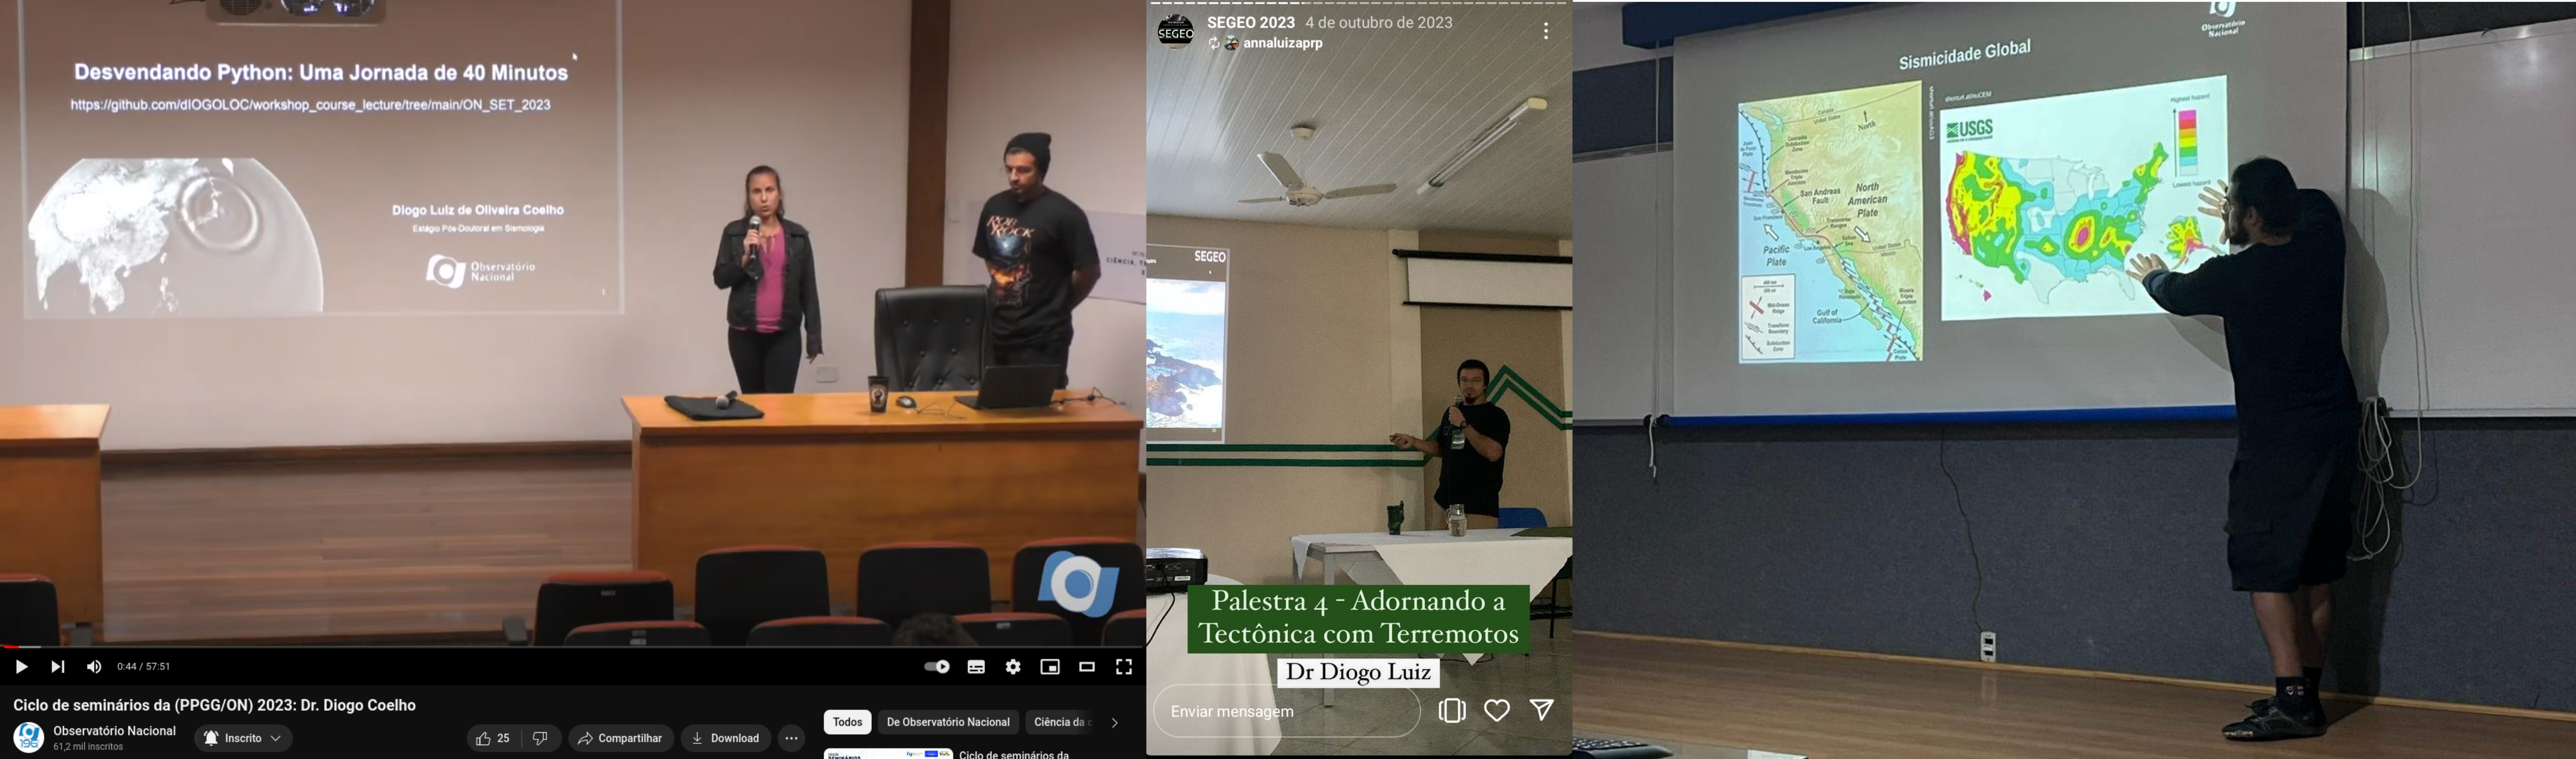
\includegraphics[width=\textwidth]{images/atuacao_ensino.png}
  \end{center}
  \caption{
    Mosaico de imagens em atividades de ensino durante o pós-doutorado no Observatório Nacional. Primeira: Ministrando um curso de python no Ciclo de Seminários do Programa de Pós-Graduação do Observatório Nacional. Segunda: Ministrando a palestra Sismologia: Adornando a Tectônica com Terremotos na Universidade Federal do Espírito Santo. Ministrando o minicurso na I Escola Itinerante da Geofísica do Observatório Nacional na Universidade Federal de Pernambuco.}
\end{figure}

\begin{summarybox}[frametitle=\faChalkboardTeacher{}\quad Resumo das atividades]
  \begin{fa-ul}
    \faStreetView & 2 orientações de alunos de iniciação científica \\
    \faBook & 1 disciplina de pós-graduação ministrada \\
    \faEdit & 3 cursos de curta duração ministrados \\
    \faNewspaper & Tópicos ensinados: Sismologia, Geologia, Tectônica, Programação (Python), Instrumentação sismológica e Geodinâmica.
  \end{fa-ul}
\end{summarybox}

As atividades de ensino e mentoria de alunos começaram formalmente apenas durante o estágio pós-doutoral. Essa falta de prática em atividades de ensino e orientação deve-se ao fato de que as bolsas de estudo concedidas para o mestrado e doutorado não exigem a realização de disciplinas ou estágios de docência. No entanto, é evidente o crescimento vertiginoso do conhecimento sismológico acumulado devido às orientações e aulas ministradas, além das oportunidades para aprender e desenvolver minhas habilidades interpessoais com outros acadêmicos. A forma de ensinar e orientar é fortemente influenciada pelas disciplinas estudadas durante a minha trajetória acadêmica, especialmente no que se refere à habilidade de selecionar e transmitir uma grande quantidade de conteúdo em um curto período de tempo. No entanto, a experiência familiar foi muito relevante neste tópico, pois a minha família é majoritariamente formada por professores da rede pública de ensino do Estado do Rio de Janeiro (\href{https://www.seeduc.rj.gov.br/}{SEEDUC}), e nas conversas informais eu aprendi diversas formas de interegir com uma turma diversa e oriunda realidades distintas. Ratificando o que foi dito anteriormente, todas as conversas com minhas tias que passaram décadas lecionando na Educação de Jovens e Adultos (\href{http://portal.mec.gov.br/index.php?option=com_docman&view=download&alias=13448-diretrizes-curiculares-nacionais-2013-pdf&Itemid=30192}{EJA}) me ajudaram a entender que a pesquisa na área das Geociências rompe com a simetria do ensino regular e impulsiona percursos individualizados, sendo a minha trajetória acadêmica um grande exemplo disso. Como a entrada no Programa de Pós-graduação em Geofísica é fomentada para uma gama de áreas do saber (e.g. graduados em Geofísica, Geologia, Física, Matemática ou áreas afins) é vital que o professor entenda a responsabilidade de estimular e viabilizar o acesso e a permanência do aluno na instituição, proporcionando oportunidades educacionais apropriadas de acordo com as características do aluno, seus interesses, condições de vida e de trabalho.

No desenvolvimento da minha prática docente, percebi que a computação é uma ferramenta poderosa para capacitar os alunos, não apenas na compreensão dos conceitos teóricos, mas também na aplicação prática desses conceitos. Através de atividades práticas, os alunos desenvolvem uma série de competências, incluindo análise de dados, resolução de problemas e pensamento crítico. Isso facilita a compreensão dos alunos e estimula sua curiosidade e interesse pelo assunto. Este capítulo oferece um breve relato das minhas atividades de ensino e orientação, destacando minha abordagem pedagógica e meu papel na ministração da disciplina de Introdução à Sismologia no Programa de Pós-graduação, onde busco promover um ambiente de aprendizado colaborativo e inclusivo, onde os alunos sintam-se capacitados a explorar e desenvolver seu potencial máximo.

\section{Orientações}
\label{sec_orientacao}

Minha primeira experiência como orientador é oriunda do Programa Institucional de Iniciação Científica e Tecnológica do ON (\href{https://www.gov.br/observatorio/pt-br/assuntos/programas-academicos/iniciacao-cientifica-e-tecnologica/apresentacao}{PICT/ON}), o qual é uma iniciativa da instituição como contrapartida ao programa de bolsas \href{http://portal-adm.cnpq.br/web/guest/pibic/}{PIBIC}, oferecido pelo Conselho Nacional de Desenvolvimento Científico e Tecnológico (\href{https://www.gov.br/cnpq/pt-br}{CNPq}). Esta iniciativa do ON ampliou o número de bolsas de Iniciação Científica e Tecnológica para alunos de graduação de diversas áreas. No entanto, um diferencial desse programa é permitir que alunos de outras universidades, localizadas fora do Rio de Janeiro, possam desenvolver trabalhos junto a pesquisadores do ON. Dada a essa nova realidade, eu iniciei a orientação das alunas \href{http://lattes.cnpq.br/4746789434324199}{Ingrid Herzog} (\href{https://unipampa.edu.br/portal/}{Unipampa}) e \href{http://lattes.cnpq.br/6698175242371919}{Thereza Mayra de Souza Fialho} (\href{https://www5.usp.br/}{USP}) inteiramente online entre Setembro de 2022 e Março de 2024 (18 meses).

O projeto realizado pela Ingrid utilizou dados das estações sismográficas situadas no estado do Rio Grande do Sul a fim de desenvolver estudos sismológicos sobre a estrutura sob essas estações, procurando correlacionar os resultados com a história geotectônica local. Nesse contexto, o método da \href{http://eqseis.geosc.psu.edu/cammon/HTML/RftnDocs/rftn01.html#:~:text=Receiver\%20functions\%20are\%20time\%20series,Earth\%20structure\%20near\%20the\%20receiver}{função do receptor} tem sido usado com sucesso para estudar descontinuidades no limite crosta/manto ao redor do mundo. Os resultados desse projeto proporcionaram informações-chave para formular hipóteses, bem como confirmar alguns modelos propostos para as grandes estruturas crustais abaixo das estações e contribuiu para ajudar a determinar os processos evolutivos que ocorreram na área de estudo. Além disso, o projeto compilou um fluxo de processamento em python para o cálculo da espessura crustal, assim como propriedades complementares oriundas da metodologia da função do receptor, que será disponibilizado para toda comunidade científica. A estudante realizou todo o processamento dos dados em algoritmos desenvolvidos em Python, utilizando os pacotes do \href{https://docs.obspy.org/}{ObsPy}, \href{https://seispy.xumijian.me/latest/}{Seispy} e \href{https://www.pygmt.org/latest/}{Pygmt}. Os resultados deste trabalhos foram satisfatórios e foram apresentados pela estudante como um resumo expandido no \href{https://sbgf.org.br/congresso/}{18 Congresso Internacional da Sociedade Brasileira de Geofísica e EXPOGEf} entre 16 e 19 de Outubro de 2023. O trabalho foi premiado pela Unipampa e a estudante foi contemplada com uma ajuda de custos para apresentar presencialmente seu pôster no congresso. Além dessa premiação, o resumo expandido recebeu a indicação para publicação no \href{https://sbgf.org.br/revista/index.php/rbgf}{Brazilian Journal of Geophysics}. Contudo, no início de 2024 recebi a notícia que a Ingrid passou no processo seletivo para mestrado no \href{https://www.iag.usp.br/}{Instituto de Astronomia, Geofísica e Ciências Atmosféricas} da USP.

o projeto realizado pela Thereza teve como objetivo comparar as particularidades dos terremotos em Marte e inferir os principais agentes causadores da sismicidade no planeta vermelho. Utilizamos a biblioteca \href{https://docs.obspy.org/}{ObsPy} para leitura e tratamento dos dados do \href{https://www.insight.ethz.ch/seismicity/catalog/v13}{catálogo sísmico da missão InSight} e, para que eles fossem mais concisos, limitamos a observação de eventos para que tivéssemos não somente a magnitude, mas também a longitude e latitude para podermos comparar com as feições geológicas existentes e, se viável, traçar um paralelo com a Terra. O grande desafio do projeto foi aplicar métodos sismológicos em dados resultantes de apenas uma estação para estudar a distribuição dos sismos marcianos, que são fortemente ofuscados pela presença de tempestades de areia e de outros processos de superfície. O âmago deste projeto foi examinar os dados contínuos do \href{https://www.iris.edu/hq/sis/insight}{InSight SEIS} para buscar entender a sismicidade em Marte através da identificação dos principais eventos sísmicos catalogados e da distribuição da atividade sísmica na superfície de Marte. Esse trabalho abriu uma nova frente de pesquisa para mim, pois os meus trabalhos e linhas de pesquisa eram relacionados à Terra. Assim como aconteceu anteriormente, a Thereza também foi aprovada no processo seletivo de mestrado do \href{https://www.iag.usp.br/}{Instituto de Astronomia, Geofísica e Ciências Atmosféricas} da USP, portanto o projeto teve que ser finalizado.

\bigskip

\begin{summarybox}[frametitle=\faBookmark{}\quad Resumo dos trabalhos apresentados pelos alunos em congressos]
  \begin{fa-ul}
      \faBuilding & 18th International Congress of the Brazilian Geophysical Society \\
      \faBook & Thickness and crustal composition investigation in the Sul-rio-grandense Shield (SrgS) \\
      \faChild & HERZOG, I.; \textbf{COELHO, D. L. O.}; HISPAGNOL, N. R. ; LIMA, M. V. A. G. D.; GREGORY, T. R.\\
      \faCertificate & \href{https://sbgf.org.br/mysbgf/eventos/expanded_abstracts/18th_CISBGf/9778d5d219c5080b9a6a17bef029331cResumo_expandd_SBGF_INGL\%C3\%8AS.docx\%20(1).pdf}{Resumo Expandido}  \\
      \faCalendar & 2023 \\
  \end{fa-ul}
\end{summarybox}

Através dessas orientações, aprendi a orientar alunos sem experiência prévia em pesquisa através das etapas iniciais de um projeto e a adaptar o nível dos projetos propostos ao nível dos alunos. Foi gratificante receber a notícia de que os alunos progrediram em suas carreiras acadêmicas e que seus projetos alcançaram uma qualidade excelente, superando até mesmo as expectativas deles mesmos.

\section{Cursos de curta duração}
\label{sec_workshops}

Minha primeira experiência em outra instituição, divulgando e ensinando sob o regime de estágio pós-doutoral no Observatório Nacional, ocorreu por convite do professor \href{http://lattes.cnpq.br/4046823088402890}{Luiz Carlos de Carvalho Benyosef}, na Escola Itinerante de Geofísica do Observatório Nacional, realizada de 08 a 10 de agosto de 2023. Foi durante esse curso que percebi minha habilidade para lecionar e divulgar a pesquisa científica. Desde então, ministrei 3 cursos de curta duração e workshops em formato online e presencial. Esses cursos complementam o ensino convencional em Sismologia e Tectônica, oferecendo a chance de explorar diferentes tecnologias, métodos de ensino e temas menos convencionais. Além disso, também ministrei cursos relacionados a integração de Sismologia e Programação em python. O formato curto é adequado para uma introdução à conceitos básicos de programação ou para abordar um assunto específico (e.g., como ler e plotar gráficos de dados sismológicos, como manipular catálogos de eventos sísmicos ou como realizar tarefas simples em python). Mesmo com um orçamento limitado é possível desenvolver esses cursos, pois atualmente existem diversas plataformas de vídeo conferência.

\bigskip

\begin{subsummarybox}[frametitle=\faEdit{}\quad Seminários e workshops ministrados]
	\begin{paperlist}
		Ago/23  & Sismologia: existem terremotos no Brasil?
		\newline
		\faInfoCircle I Escola Itinerante de Geofísica do Observatório Nacional (presencial).
		\newline
		\faBuilding Universidade Federal de Pernambuco  (Recife-PE)
		\newline
		\faArchive{} \href{https://doi.org/10.6084/m9.figshare.25387180.v1}{Apresentação}
		\faBullhorn{} \href{https://www.ufpe.br/df/todos-os-informes/-/asset_publisher/znKKONCGSp59/content/a-primeira-escola-itinerante-de-geofisica-do-observatorio-nacional-ocorrera-na-ufpe-no-periodo-de-08-10-de-agosto-de-2023/441331}{Noticia}
		\\
		Set/23  & Desvendando Python: Uma Jornada de 40 Minutos.
		\newline
		\faInfoCircle Ciclo de seminários do PPGG/ON 2023 (presencial/online)
		\newline
		\faBuilding Observatório Nacional (Rio de Janeiro-RJ) 
		\newline
		\faGithub{} \href{https://github.com/dIOGOLOC/workshop_course_lecture/tree/6a0758f18303eecb6344a61fdbf874225da5e6be/ON_SET_2023}{Código}
		\faYoutube{} \href{https://youtu.be/LhRH2uYTWhc}{Vídeo}
		\\ 
		Out/23 & Sismologia e Python: Introdução prática ao processamento de dados sismológicos
		\newline
		\faInfoCircle XI Semana de Estudos Geológicos da Universidade Federal do Espírito Santo/IX Semana de Geologia do Espírito Santo (presencial)
		\newline
		\faBuilding Universidade Federal do Espírito Santo (Alegre-ES) 
		\newline
		\faArchive{} \href{https://doi.org/10.6084/m9.figshare.25387123.v1}{Apresentação}
		\faGithub{} \href{https://github.com/dIOGOLOC/workshop_course_lecture/tree/6a0758f18303eecb6344a61fdbf874225da5e6be/SEGEO_2023_UFES}{Código}
		\\
	\end{paperlist}
\end{subsummarybox}

\section{Disciplinas na pós-graduação}
\label{sec_ensino_grad}

Sou o responsável, juntamente com o professor \href{http://lattes.cnpq.br/8537150955145617}{Sergio Luiz Fontes}, pela disciplina \href{https://www.gov.br/observatorio/pt-br/assuntos/programas-academicos/pos-graduacao-em-geofisica/ementas/introducao-a-sismologia}{Introdução à Sismologia} onde ensino de maneira introdutória terremotos, estrutura da Terra, aquisição e processamento de dados sísmicos e instrumentação dentro nos diversos campos de atuação da \href{http://www.rsis.on.br/}{Rede Sismográfica do Sul e do Sudeste do Brasil (RSIS)}. Dada a complexidade da mecânica de terremotos e da geodinânima, aliados ao pouco tempo disponível para a disciplina (3 meses), o processo de avaliação utilizado para mensurar o desempenho dos alunos está relacionado a confecção de três tipos de resumos (e.g. informativo, indicativo e crítico) sobre artigos científicos da área. A proposta desse processo de avaliação\footnote{Exemplos: avaliações \href{https://docs.google.com/forms/d/e/1FAIpQLSffa78ttrM_i5cWZmISGNz-lhwShi3Wzk7AUbWPgN6lhDuTNQ/viewform}{2} e \href{https://docs.google.com/forms/d/e/1FAIpQLSe8FIH4vSjn5QLT79BdG8eVRLti0le8i6yssInmQTX1iXNrYA/viewform}{3}} é ensinar aos alunos a elaboração de um resumo científico, tanto em português quanto em inglês, já que para a maioria deles, essa seria sua primeira experiência e contato com a escrita científica. Além disso, incorporei uma abordagem computacional introduzindo a manipulação de tabelas e dados de eventos sísmicos dentro do ambiente do \href{https://colab.google/}{google colab}, que é um serviço hospedado do \href{https://jupyter.org/}{Jupyter Notebook} que não requer configuração para ser usado e fornece acesso gratuito a recursos de computação. O Colab é especialmente adequado para aprendizado de máquina, ciência de dados e educação computacional básica. Como exemplos temos a \href{https://colab.research.google.com/drive/1c7Vc_s0A5GURJIab2vTS-LCW8fPlRaXt?usp=sharing}{aula de introdução ao Google colab} e a \href{https://colab.research.google.com/drive/17VaW0MkQxcxUjGaeowaVwyRORrijCXaV?usp=sharing}{aula de introdução ao Python}.

\bigskip

\begin{subsummarybox}[frametitle=\faGraduationCap{}\quad Disciplinas ministradas no Observatório Nacional]
  \begin{courselist}
    2022--2024 &
      SISMO - Introdução à Sismologia
      \newline
      \faInfoCircle \href{https://www.gov.br/observatorio/pt-br/assuntos/programas-academicos/pos-graduacao-em-geofisica/grade-curricular}{Grade Curricular}
      \newline
      \faInbox \href{https://www.gov.br/observatorio/pt-br/assuntos/programas-academicos/pos-graduacao-em-geofisica/ementas/introducao-a-sismologia}{Ementa}
  \end{courselist}
\end{subsummarybox}

Estou plenamente disponível e comprometido para ministrar essas novas disciplinas de Sismologia na pós-graduação. Com uma sólida experiência em pesquisa e análise de dados sísmicos, estou entusiasmado em oferecer aos alunos uma educação de alta qualidade e prepará-los para os desafios do mundo real. Estou confiante para trabalhar em colaboração com os alunos para promover uma compreensão profunda e abrangente da sismologia e suas aplicações.

%==============================================================================


\chapter{Popularização da Ciência}
\label{cap_comunidade}

\bigskip

\begin{figure}[h]
  \HeroFigPad
  \begin{center}
    \includegraphics[width=\textwidth]{images/atuacao_divulga.png}
  \end{center}
  \caption{
    Mosaico mostrando as diversas frentes de atuação na divulgação e popularização da ciência durante o estágio pós-doutoral no Observatório Nacional. Esquerda: Participação com o Projeto Sismo-oceanográfico em 2022 no Rio Innovation Week. Centro: 3 fotos de entrevistas respondendo os questionamentos da sociedade em relação a sismicidade brasileira e global. Direita: Ministrando o mini-curso \textit{Sismologia: existem terremotos no Brasil?} na Universidade Federal de Pernambuco.}
\end{figure}

Após ingressar no estágio pós-doutoral, cerca de um mês depois, o planeta iniciou um extenso período de \href{http://repositoriocovid19.unb.br/repositorio-produtos/desvelando-o-isolamento-social-no-cotidiano-vivido-na-pandemia-da-covid-19/}{isolamento social}. Foi nesse contexto que constatei uma crescente demanda social por informações científicas verídicas, além de identificar uma lacuna significativa em minha carreira no campo da divulgação científica, área que ganhou um destaque gigantesco na ciência contemporânea. Diante dessa necessidade evidente, iniciei minhas atividades voltadas para à divulgação e popularização da ciência junto à Divisão de Comunicação e Popularização da Ciência (\href{https://www.gov.br/observatorio/pt-br/assuntos/areas-de-atuacao/divulgacao-e-popularizacao-da-ciencia}{DICOP}), reconhecendo a importância de fornecer conhecimento acessível à sociedade. Este capítulo relata minhas atividades relacionadas à divulgação da ciência, como mostra a Figura \ref{fig_resumo_divulgacao}. Durante esse período, meu engajamento abrangeu a diversas demandas da DICOP em variadas plataformas de comunicação, abordando tanto o meio virtual, por meio de redes sociais e canais de imprensa online, quanto atividades presenciais, como feiras e eventos de divulgação científica e tecnológica, assim que as restrições permitiram.

\begin{figure}
	\centering
	\begin{tikzpicture}
	\pie{34.3/Entrevista escrita (13),
		21.0/Entrevista gravada (8),
		10.5/Revisão de texto (4),
		7.8/Evento Online (3), 
		7.8/Entrevista ao vivo (3),
		5.2/Evento presencial (2),
		5.2/Mini-curso (2),
		8/Outros (3)}
	\end{tikzpicture}
	\caption{Estatística das atividades de divulgação científicas realizadas entre 2020 e 2024.}
	\label{fig_resumo_divulgacao}˘
\end{figure}

Os números apresentados acima, assim como a lista \ref{lista_divulgacao}, fornecem uma visão detalhada dessa abordagem multifacetada na popularização da ciência e das atividades do Obseravtório Nacional ao longo do período que estive na instituição, um total de 38 atividades ao longo de 3 anos. Destaco que concedi dezenas de entrevistas, totalizando 24 (13 escritas, 8 gravadas e 3 ao vivo), contribuí revisando textos na temática da Sismologia e Geologia que foram publicados nas redes sociais do Observatório Nacional. Além disso, fiz parte da comitiva que participou do \href{https://www.gov.br/observatorio/pt-br/assuntos/areas-de-atuacao/divulgacao-e-popularizacao-da-ciencia/on-riw}{Rio Innovation Week}, o maior evento de tecnologia e inovação da América Latina, para apresentar as iniciativas, ações e projetos ligados ao \href{https://www.gov.br/mcti/pt-br}{MCTI}. Somado a isso, ministrei dois minicursos em duas instituições de ensino superior, na Universidade Federal do Espírito Santo para o curso de Geologia na \href{https://www.instagram.com/segeo.ufes/}{Semana de Estudos Geológicos da Universidade Federal do Espírito Santo} e no Instituto de Física da Universidade Federal de Pernambuco na \href{https://www.gov.br/observatorio/pt-br/assuntos/noticias/i-escola-itinerante-da-geofisica-do-observatorio-nacional-e-realizada-na-ufpe}{I Escola Itinerante da Geofísica do Observatório Nacional}. Ministrar um curso em outras instituições, não apenas promove a disseminação do conhecimento especializado, mas também desempenha um papel crucial na visibilidade e reputação do Observatório Nacional. Esses eventos compartilham expertise em contextos acadêmicos diversos, estabelecendo laços colaborativos e fortalecendo a presença no cenário acadêmico. Além disso, o envolvimento em eventos externos fortalece parcerias e colabora para o crescimento do programa de iniciação científica e pós-graduação do ON, estimulando a atração de novos alunos.

\bigskip

\begin{subsummarybox}[frametitle=\faList{}\quad Listagem das atividades de divulgação científica]
  \label{lista_divulgacao}
  \begin{datelist}
  	06/05/2020 & Evento Online - Youtube ON - \href{https://youtu.be/TrTe2VveEB8}{Diminuição do zumbido urbano no planeta} \\
	13/05/2020 & Entrevista gravada - Ciência na Rádio - \href{https://www.gov.br/observatorio/pt-br/acesso-a-informacao/auditorias/relatorios-do-termo-de-compromisso-de-gestao/documentos/on_relatorio_tcg_2020.pdf/view}{Diminuímos o zumbido urbano no planeta} \\
	01/09/2020 & Evento Online - Youtube ON - \href{https://youtu.be/dHavR6DvAIo}{A terra tremeu na Bahia!}\\
	09/09/2020 & Entrevista gravada - Ciência na Rádio - \href{https://www.gov.br/observatorio/pt-br/acesso-a-informacao/auditorias/relatorios-do-termo-de-compromisso-de-gestao/documentos/on_relatorio_tcg_2020.pdf/view}{Tremores de terra na Bahia}\\
	30/08/2020 & Entrevista ao vivo - GloboNews - \href{https://g1.globo.com/globonews/jornal-globonews/video/magnitude-choca-um-pouco-as-pessoas-diz-sismologo-sobre-terremoto-na-bahia-8817616.ghtml}{"Magnitude choca um pouco as pessoas", diz sismólogo sobre terremoto na Bahia}\\
	29/04/2021 & Evento Online - Youtube ON - \href{https://youtu.be/Zazh2MlbkXU}{Por que a terra treme no Brasil?}\\
	05/07/2021 & Revisão de texto - Facebook ON - \href{https://www.facebook.com/observatorionacional/videos/319161219946539}{você pode conhecer um pouco mais sobre a sismologia, que é o estudo dos terremotos e da estrutura da Terra.}\\		
	21/07/2021 & Entrevista gravada - Ciência na Rádio - \href{https://radios.ebc.com.br/radio-sociedade/2021/07/o-mar-tambem-treme-nao-so-terra}{O mar também treme, não só a terra} \\
	26/07/2021 & Entrevista escrita - apufsc - \href{https://www.apufsc.org.br/2021/07/26/equipe-da-ufsc-trabalha-com-dados-ineditos-captados-por-equipamentos-complexos-instalados-no-fundo-do-oceano/}{Equipe da UFSC trabalha com dados inéditos captados por equipamentos complexos instalados no fundo do oceano}\\	
	26/07/2021 & PodCast - IFFcast - \href{https://podcasters.spotify.com/pod/show/iffcast/episodes/66-Terremotos-e150eb0/a-a67a2kg}{66 Terremotos}\\	
	26/07/2021 & Entrevista escrita - Noticias UFSC - \href{https://noticias.ufsc.br/2021/07/equipe-da-ufsc-trabalha-com-dados-ineditos-captados-por-equipamentos-complexos-instalados-no-fundo-do-oceano/}{Equipe da UFSC trabalha com dados inéditos captados por equipamentos complexos instalados no fundo do oceano}\\	
	27/07/2021 & Entrevista escrita - FAPEU - \href{http://www.fapeu.com.br/noticias.php?id_noticia=351\&id_categoria=5}{Projeto apoiado pela UFSC trabalha com dados inéditos captados por equipamentos instalados no fundo do oceano}\\	
	10/10/2021 & Entrevista ao vivo - JAM - \href{https://globoplay.globo.com/v/10614041/}{Moradores relatam tremor em Manaus após terremoto no Peru}\\
	17/10/2021 & Entrevista gravada - Ciência na Rádio - \href{https://radios.ebc.com.br/radio-sociedade/2021/10/cumbre-vieja-maior-erupcao-vulcanica-na-europa-em-100-anos}{Cumbre Vieja, a maior erupção vulcânica na Europa em 100 anos}\\
	13/01/2022 & Entrevista escrita - Site ON - \href{https://www.gov.br/observatorio/pt-br/assuntos/areas-de-atuacao/divulgacao-e-popularizacao-da-ciencia/on-riw/monitoramento-de-tremores-de-terra-no-brasil-1}{Projeto de monitoramento sismo-oceanográfico e RSBR}\\	
	13/01/2022 & Evento presencial - Rio Innovation Week - \href{https://www.gov.br/observatorio/pt-br/assuntos/areas-de-atuacao/divulgacao-e-popularizacao-da-ciencia/on-riw}{Participação com o Projeto Sismo-oceanográfico na Rio Innovation Week. O evento ocorreu entre os dias 13 e 16 de janeiro de 2022.}\\	
	02/02/2022 & Revisão de texto - Facebook ON - \href{https://www.facebook.com/photo?fbid=4569504043159191\&set=a.318827624893542}{Os cânions são formações rochosas impressionantes!}\\	
	04/03/2022 & Entrevista gravada - Ciência na Rádio - \href{https://radios.ebc.com.br/radio-sociedade/2022/03/entenda-o-que-sao-movimentos-de-massa-inundacoes-e-quais-sao-os-impactos}{Podcast: como os desastres ambientais são causados}\\
	26/05/2022 & Revisão de texto - Facebook ON - \href{https://www.facebook.com/photo?fbid=314008907578314\&set=a.279769034335635}{Um terremoto de magnitude 7,2 atingiu o Peru nesta quinta-feira (26) e pôde ser sentido em Manaus (AM).}\\	
	03/06/2022 & Entrevista escrita - O Tempo - \href{https://www.otempo.com.br/super-noticia/sete-lagoas-investiga-serie-de-tremores-de-terra-1.2678079}{Sete Lagoas investiga série de tremores de terra}\\
	04/09/2022 & Palestra Online - \href{https://youtu.be/yTUVBx0fsDA}{107ª QCC - Monitoramento sísmico marinho no Brasil - Diogo Coelho (ON)}\\
	08/11/2022 & Evento presencial - Rio Innovation Week - \href{https://www.gov.br/observatorio/pt-br/assuntos/noticias/observatorio-nacional-leva-ciencia-e-tecnologia-ao-rio-innovation-week-2022}{Observatório Nacional (ON/MCTI) leva ciência e tecnologia à Rio Innovation Week entre 8 e 11 de novembro de 2022}\\	
	14/12/2022 & Entrevista gravada - Ciência na Rádio - \href{https://radios.ebc.com.br/radio-sociedade/2022/12/impacto-de-navio-deriva-na-ponte-rio-niteroi-foi-equivalente-um-terremoto-de}{Impacto de navio a deriva na Ponte Rio-Niterói foi equivalente a terremoto de magnitude 1.6}\\
	19/12/2022 & Entrevista escrita - Enfoco - \href{https://enfoco.com.br/noticias/cidades/colisao-de-navio-com-a-ponte-rio-niteroi-provoca-terremoto-video-88684?d=1}{Colisão de navio com a Ponte Rio-Niterói provoca terremoto}\\
	06/02/2023 & Revisão de texto - Facebook ON - \href{https://www.facebook.com/photo?fbid=504786468504778\&set=a.286674090316018}{Você deve ter lido recentemente que o núcleo da Terra pode se inverter.}\\	
	10/02/2023 & Entrevista escrita - Enfoque MS - \href{https://www.enfoquems.com.br/estudo-aponta-que-nucleo-da-terra-desacelerou-e-fenomeno-pode-afetar-duracao-dos-dias/}{Estudo aponta que núcleo da Terra desacelerou, e fenômeno pode afetar duração dos dias}\\
	11/02/2023 & Entrevista gravada - Jovem Pan News - \href{https://youtu.be/MlcSJgjTF7A}{Terremoto Turquia | DOCUMENTO JOVEM PAN - 11/02/2023}\\
	27/02/2023 & Entrevista escrita - Jornal Força do Vale - \href{https://jornalforcadovale.com.br/mundo/como-cientistas-estudam-a-importancia-do-nucleo-da-terra/}{Como cientistas estudam a importância do núcleo da Terra}\\
	24/04/2023 & Entrevista escrita - Site ON - \href{https://www.gov.br/observatorio/pt-br/assuntos/noticias/on-investiga-terremotos-antigos-na-regiao-do-pre-sal-com-veiculo-subaquatico-autonomo\#:~:text=Pesquisadores\%20da\%20\%C3\%A1rea\%20de\%20geof\%C3\%ADsica,de\%20explora\%C3\%A7\%C3\%A3o\%20do\%20Pr\%C3\%A9\%2DSal.}{ON investiga terremotos antigos na região do Pré-Sal com ‘veículo subaquático autônomo’}\\
	26/04/2023 & Entrevista gravada - Ciência na Rádio - \href{https://radios.ebc.com.br/radio-sociedade/2023/04/entenda-o-uso-de-veiculos-subaquaticos-na-descoberta-de-terremotos-antigos}{Entenda o uso de veículos subaquáticos na descoberta de terremotos antigos}\\
	08/08/2023 & Workshop - UFPE - \href{https://www.gov.br/observatorio/pt-br/assuntos/noticias/i-escola-itinerante-da-geofisica-do-observatorio-nacional-e-realizada-na-ufpe}{I Escola Itinerante da Geofísica do Observatório Nacional}\\
	14/09/2023 & Entrevista ao vivo - CNN Pop - \href{https://youtu.be/NqFl7g9YMsE}{Vulcão Kilauea entra em erupção pela 3ª vez em 2023: como o fenômeno acontece? | Popverso CNN}\\
	02/10/2023 & Palestra Presencial - SEGEO/UFES - \href{https://www.instagram.com/segeo.ufes/}{Sismologia: Adornando a Tectônica com Terremotos}\\
	22/01/2024 & Entrevista escrita - Site ON - \href{https://www.gov.br/observatorio/pt-br/assuntos/noticias/sismologo-do-observatorio-nacional-explica-terremoto-registrado-pela-rede-sismografica-brasileira-no-norte-do-brasil?fbclid=IwAR2a42LyCxwwkI93V6Axrv9bB2AR8Pdx6IqMW2tPlzkwZIcrE18Jq9aU39U}{Sismólogo do Observatório Nacional explica terremoto registrado pela Rede Sismográfica Brasileira no Norte do Brasil}\\
	24/01/2024 & Entrevista escrita - Canaltech - \href{https://canaltech.com.br/meio-ambiente/por-que-ninguem-sentiu-o-terremoto-de-66-graus-no-brasil-276873/}{Por que ninguém sentiu o terremoto de 6,6 graus no Brasil?}\\
	01/02/2024 & Entrevista escrita - Canaltech - \href{https://canaltech.com.br/meio-ambiente/da-para-prever-um-terremoto-com-antecedencia/}{Dá para prever um terremoto com antecedência?} \\
	11/02/2024 & Entrevista escrita - Multiverso Noticias - \href{https://multiversonoticias.com.br/terremoto-no-brasil-descubra-quais-regioes-sao-mais-vulneraveis/}{Terremoto no Brasil: descubra quais regiões são mais vulneráveis}\\
  \end{datelist}
\end{subsummarybox}

%==============================================================================

\chapter{Considerações Finais}
\label{cap_conclusao}

Este memorial narra minha jornada desde os meados dos anos 2000, quando iniciei meu curso de Geologia na Universidade Federal do Espírito Santo, até meu último estágio pós-doutoral no Observatório Nacional, instituição que desempenhou um papel fundamental ao longo da minha trajetória acadêmica. Durante meu último estágio pós-doutoral nessa instituição, pude aprofundar meu conhecimento e contribuir para projetos de pesquisa de grande relevância. Nessa maratona acadêmica, passei por 4 instituições federais em 4 estados diferentes, visitei 15 estados para participar de conferências nacionais e aulas de campo e visitei 5 países assistindo a cursos e conferências internacionais graças às oportunidades geradas pelos programas de pós-graduação, projetos e bolsas que estive envolvido.

Atuo em diversas linhas de pesquisa relacionadas à Sismologia, com aplicações na indústria e na academia. Toda a minha caminhada estive envolvido à tópicos da sismologia, no entanto, sempre estive aberto a coloborar com outras áreas. A experiência na Sismologia Marinha mostrou minha habilidade multidisciplinar com outras áreas das Ciências Marinhas. Todo o ensino superior, de alta qualidade, foi-me proporcionado de forma gratuita e através de inúmeros auxílios para estudos na pós-graduação. Se houver a possibilidade, estou pronto para retribuir com a experiência que adquiri em pesquisa, ensino e divulgação científica. Caso tenha a oportunidade, pretendo buscar colaborações com os pesquisadores e pesquisadoras do Observatório Nacional e de outras instituições na região Sudeste, no Brasil e na América do Sul, inicialmente. Posteriormente, a vontade é de consolidar colaborações com outras regiões do mundo. As áreas de atuação são diversas, como estrutura da Terra, regionalmente e globalmente, monitoramento sísmico e acústico, tectônica e de instrumentação geofísica. No quesito do ensino, eu tenho a capacidade de ajudar a pós-graduação em diversos tópicos que ligam a Geologia, Geofísica e Sismologia, propondo disciplinas eletivas, cursos de aperfeiçoamento e cursos de curta duração. Além disso, atualmente existe a expansão da utilização de ferramentas remotas para o ensino, aperfeiçoamento e divulgação da Ciência. 

Desde os dias de estudante de graduação até o estágio pós-doutoral no Observatório Nacional, tenho vivenciado uma jornada repleta de descobertas, desafios, derrotas e conquistas, que não só moldaram minha carreira acadêmica, mas ampliaram minha visão de mundo e fortaleceram meu compromisso com a excelência na pesquisa e inovação científica. Durante esse percurso, o conhecimento adquirido me ajudou a vislubar bons direcionamentos na carreira acadêmica. Essa experiência me fez perceber as lacunas no meu ensino e a necessidade de me dedicar mais e buscar a colaboração de outro pesquisadores para melhorar as perguntas e respostas para cada linha de pesquisa. Em suma, seria uma honra ter a oportunidade de contribuir com a instituição, formando novos pesquisadores, conduzindo pesquisas inovadoras e ampliando o leque de possibilidades de serviços prestados à sociedade.

\end{document}
